% Options for packages loaded elsewhere
\PassOptionsToPackage{unicode}{hyperref}
\PassOptionsToPackage{hyphens}{url}
\documentclass[
]{article}
\usepackage{xcolor}
\usepackage[margin=1in]{geometry}
\usepackage{amsmath,amssymb}
\setcounter{secnumdepth}{-\maxdimen} % remove section numbering
\usepackage{iftex}
\ifPDFTeX
  \usepackage[T1]{fontenc}
  \usepackage[utf8]{inputenc}
  \usepackage{textcomp} % provide euro and other symbols
\else % if luatex or xetex
  \usepackage{unicode-math} % this also loads fontspec
  \defaultfontfeatures{Scale=MatchLowercase}
  \defaultfontfeatures[\rmfamily]{Ligatures=TeX,Scale=1}
\fi
\usepackage{lmodern}
\ifPDFTeX\else
  % xetex/luatex font selection
\fi
% Use upquote if available, for straight quotes in verbatim environments
\IfFileExists{upquote.sty}{\usepackage{upquote}}{}
\IfFileExists{microtype.sty}{% use microtype if available
  \usepackage[]{microtype}
  \UseMicrotypeSet[protrusion]{basicmath} % disable protrusion for tt fonts
}{}
\makeatletter
\@ifundefined{KOMAClassName}{% if non-KOMA class
  \IfFileExists{parskip.sty}{%
    \usepackage{parskip}
  }{% else
    \setlength{\parindent}{0pt}
    \setlength{\parskip}{6pt plus 2pt minus 1pt}}
}{% if KOMA class
  \KOMAoptions{parskip=half}}
\makeatother
\usepackage{color}
\usepackage{fancyvrb}
\newcommand{\VerbBar}{|}
\newcommand{\VERB}{\Verb[commandchars=\\\{\}]}
\DefineVerbatimEnvironment{Highlighting}{Verbatim}{commandchars=\\\{\}}
% Add ',fontsize=\small' for more characters per line
\usepackage{framed}
\definecolor{shadecolor}{RGB}{248,248,248}
\newenvironment{Shaded}{\begin{snugshade}}{\end{snugshade}}
\newcommand{\AlertTok}[1]{\textcolor[rgb]{0.94,0.16,0.16}{#1}}
\newcommand{\AnnotationTok}[1]{\textcolor[rgb]{0.56,0.35,0.01}{\textbf{\textit{#1}}}}
\newcommand{\AttributeTok}[1]{\textcolor[rgb]{0.13,0.29,0.53}{#1}}
\newcommand{\BaseNTok}[1]{\textcolor[rgb]{0.00,0.00,0.81}{#1}}
\newcommand{\BuiltInTok}[1]{#1}
\newcommand{\CharTok}[1]{\textcolor[rgb]{0.31,0.60,0.02}{#1}}
\newcommand{\CommentTok}[1]{\textcolor[rgb]{0.56,0.35,0.01}{\textit{#1}}}
\newcommand{\CommentVarTok}[1]{\textcolor[rgb]{0.56,0.35,0.01}{\textbf{\textit{#1}}}}
\newcommand{\ConstantTok}[1]{\textcolor[rgb]{0.56,0.35,0.01}{#1}}
\newcommand{\ControlFlowTok}[1]{\textcolor[rgb]{0.13,0.29,0.53}{\textbf{#1}}}
\newcommand{\DataTypeTok}[1]{\textcolor[rgb]{0.13,0.29,0.53}{#1}}
\newcommand{\DecValTok}[1]{\textcolor[rgb]{0.00,0.00,0.81}{#1}}
\newcommand{\DocumentationTok}[1]{\textcolor[rgb]{0.56,0.35,0.01}{\textbf{\textit{#1}}}}
\newcommand{\ErrorTok}[1]{\textcolor[rgb]{0.64,0.00,0.00}{\textbf{#1}}}
\newcommand{\ExtensionTok}[1]{#1}
\newcommand{\FloatTok}[1]{\textcolor[rgb]{0.00,0.00,0.81}{#1}}
\newcommand{\FunctionTok}[1]{\textcolor[rgb]{0.13,0.29,0.53}{\textbf{#1}}}
\newcommand{\ImportTok}[1]{#1}
\newcommand{\InformationTok}[1]{\textcolor[rgb]{0.56,0.35,0.01}{\textbf{\textit{#1}}}}
\newcommand{\KeywordTok}[1]{\textcolor[rgb]{0.13,0.29,0.53}{\textbf{#1}}}
\newcommand{\NormalTok}[1]{#1}
\newcommand{\OperatorTok}[1]{\textcolor[rgb]{0.81,0.36,0.00}{\textbf{#1}}}
\newcommand{\OtherTok}[1]{\textcolor[rgb]{0.56,0.35,0.01}{#1}}
\newcommand{\PreprocessorTok}[1]{\textcolor[rgb]{0.56,0.35,0.01}{\textit{#1}}}
\newcommand{\RegionMarkerTok}[1]{#1}
\newcommand{\SpecialCharTok}[1]{\textcolor[rgb]{0.81,0.36,0.00}{\textbf{#1}}}
\newcommand{\SpecialStringTok}[1]{\textcolor[rgb]{0.31,0.60,0.02}{#1}}
\newcommand{\StringTok}[1]{\textcolor[rgb]{0.31,0.60,0.02}{#1}}
\newcommand{\VariableTok}[1]{\textcolor[rgb]{0.00,0.00,0.00}{#1}}
\newcommand{\VerbatimStringTok}[1]{\textcolor[rgb]{0.31,0.60,0.02}{#1}}
\newcommand{\WarningTok}[1]{\textcolor[rgb]{0.56,0.35,0.01}{\textbf{\textit{#1}}}}
\usepackage{longtable,booktabs,array}
\usepackage{calc} % for calculating minipage widths
% Correct order of tables after \paragraph or \subparagraph
\usepackage{etoolbox}
\makeatletter
\patchcmd\longtable{\par}{\if@noskipsec\mbox{}\fi\par}{}{}
\makeatother
% Allow footnotes in longtable head/foot
\IfFileExists{footnotehyper.sty}{\usepackage{footnotehyper}}{\usepackage{footnote}}
\makesavenoteenv{longtable}
\usepackage{graphicx}
\makeatletter
\newsavebox\pandoc@box
\newcommand*\pandocbounded[1]{% scales image to fit in text height/width
  \sbox\pandoc@box{#1}%
  \Gscale@div\@tempa{\textheight}{\dimexpr\ht\pandoc@box+\dp\pandoc@box\relax}%
  \Gscale@div\@tempb{\linewidth}{\wd\pandoc@box}%
  \ifdim\@tempb\p@<\@tempa\p@\let\@tempa\@tempb\fi% select the smaller of both
  \ifdim\@tempa\p@<\p@\scalebox{\@tempa}{\usebox\pandoc@box}%
  \else\usebox{\pandoc@box}%
  \fi%
}
% Set default figure placement to htbp
\def\fps@figure{htbp}
\makeatother
\setlength{\emergencystretch}{3em} % prevent overfull lines
\providecommand{\tightlist}{%
  \setlength{\itemsep}{0pt}\setlength{\parskip}{0pt}}
\usepackage{bookmark}
\IfFileExists{xurl.sty}{\usepackage{xurl}}{} % add URL line breaks if available
\urlstyle{same}
\hypersetup{
  pdftitle={Dashboards for Clicker Data},
  pdfauthor={{[}{[}Team Night Owl, Kayla Runkel (kmr227), Gianna Ou (gyo4), Shiwen Zhao (sz752), Theo Berk (tb547), Maisha Farzana (maf372), and Steven Xie (jx453){]}{]}},
  hidelinks,
  pdfcreator={LaTeX via pandoc}}

\title{Dashboards for Clicker Data}
\usepackage{etoolbox}
\makeatletter
\providecommand{\subtitle}[1]{% add subtitle to \maketitle
  \apptocmd{\@title}{\par {\large #1 \par}}{}{}
}
\makeatother
\subtitle{INFO 4100 Learning Analytics}
\author{{[}{[}Team Night Owl, Kayla Runkel (kmr227), Gianna Ou (gyo4),
Shiwen Zhao (sz752), Theo Berk (tb547), Maisha Farzana (maf372), and
Steven Xie (jx453){]}{]}}
\date{}

\begin{document}
\maketitle

This project is about developing a learning analytics dashboard based on
clicker data. You will work as a team to learn how to make a dashboard
using R Shiny (official page with several tutorials:
\url{https://shiny.rstudio.com/tutorial/}).

\textbf{Learning Objectives}

\begin{enumerate}
\def\labelenumi{\arabic{enumi}.}
\tightlist
\item
  Understand the structure of clicker data
\item
  Create multiple different visualizations
\item
  Design and implement an instructor and student dashboard
\item
  Critically evaluate your own dashboard design
\end{enumerate}

You are given aggregated clicker records for a CS course taught at
Cornell. There are two datasets: the experience dataset and the quiz
dataset.

\textbf{Scenario}

You are approached by a college instructor who uses iClickers in her CS
class on Business Intelligence. She would like to gain insights about
her students and how they are engaging/performing in order to better
help them in class. She would also like to better support students by
giving them feedback at scale about where they stand and perhaps how
they compare to others in the class.

You offer to build a prototype of a dashboard using her clicker data:
this is a dashboard for the instructor which offers an overview of the
class characteristics, engagement, and performance; and it is a
dashboard for students which offers a specific student an overview of
their engagement and performance (and how it compares to others).

\textbf{Data}

The \textbf{experience dataset} contains one record per student who
completed the CS course between 2016-2018. There are two sources to this
dataset: Faculty Center and a Skills Survey (administered via the
Blackboard LMS) where students self reported their skill level for
various skills the first week of class. This data has been
de-identified. Name, netid, emplid, major have all been removed and
replaced with a unique numeric identifier. Note that not all students
completed the skills survey, they will have null values for the survey
result fields.

\begin{longtable}[]{@{}
  >{\raggedright\arraybackslash}p{(\linewidth - 4\tabcolsep) * \real{0.3333}}
  >{\raggedright\arraybackslash}p{(\linewidth - 4\tabcolsep) * \real{0.3333}}
  >{\raggedright\arraybackslash}p{(\linewidth - 4\tabcolsep) * \real{0.3333}}@{}}
\toprule\noalign{}
\begin{minipage}[b]{\linewidth}\raggedright
Attribute Name
\end{minipage} & \begin{minipage}[b]{\linewidth}\raggedright
Data Type
\end{minipage} & \begin{minipage}[b]{\linewidth}\raggedright
Definition
\end{minipage} \\
\midrule\noalign{}
\endhead
\bottomrule\noalign{}
\endlastfoot
student\_key & numeric Unique key & Assigned as part of
de-identification process. Uniquely identifies student records for this
data set only. \\
year & numeric & Four digit year student was enrolled in BI Class. \\
prog & character Values (GRAD, UGRAD) & Indicates whether the student
was a graduate or undergraduate student when they were enrolled in BI
course. \\
database\_score & numeric (0-5) & Self reported experience level with
database technology prior to taking course. 0= no experience, 5=
expertise \\
sql\_score & numeric (0-5) & Self reported experience level with SQL
prior to taking course. 0= no experience, 5=expertise \\
programing\_score & numeric (0-5) & Self reported experience level with
Any Programing language prior to taking course. 0=no experience,
5=expertise \\
stored\_proc\_score & numeric (0-5) & Self reported experience level
with stored procedure languages prior to taking course. 0=no experience,
5=expertise \\
etl\_score & numeric (0-5) & Self reported experience level with Extract
Transform Load (ETL) development prior to taking course. 0=no
experience, 5=expertise \\
data\_vis\_score & numeric (0-5) & Self reported experience level using
data visualization tools prior to taking course. 0=no experience,
5=expertise \\
requirement\_gather\_score & numeric (0-5) & Self reported experience
level gathering customer requirements prior to taking course. 0=no
experience, 5=expertise \\
skill\_survey\_score & numeric & Sum of the self reported skill level
scores. \\
\end{longtable}

The \textbf{quiz dataset} contains one record per student per class
session held where iClickers were used. Sources used in the creation of
this data set include: iClicker session xml files, Blackboard gradebook
(for quiz scores), and the Blackboard class schedule (used to map
iClicker session to related quiz scores). Note that in some cases there
are multiple iClicker sessions / lectures associated with a single quiz.
This dataset may be joined to the experience dataset by the student\_key
field.

\begin{longtable}[]{@{}
  >{\raggedright\arraybackslash}p{(\linewidth - 4\tabcolsep) * \real{0.3333}}
  >{\raggedright\arraybackslash}p{(\linewidth - 4\tabcolsep) * \real{0.3333}}
  >{\raggedright\arraybackslash}p{(\linewidth - 4\tabcolsep) * \real{0.3333}}@{}}
\toprule\noalign{}
\begin{minipage}[b]{\linewidth}\raggedright
Attribute Name
\end{minipage} & \begin{minipage}[b]{\linewidth}\raggedright
Data Type
\end{minipage} & \begin{minipage}[b]{\linewidth}\raggedright
Definition
\end{minipage} \\
\midrule\noalign{}
\endhead
\bottomrule\noalign{}
\endlastfoot
Acad\_date\_key & numeric & Date key in the form of YYYYMMDD indicating
the date the class session was held. \\
student\_key & numeric & Unique identifier for students who took BI
class 2016-2018. This key is the primary key for the experience\_data
file. \\
year & numeric & Four digit year class session was held. \\
session\_number & numeric & Identifies the session number for a
particular semester. Session number is assigned by iClicker. \\
quiz\_number & numeric & There are 10 quizzes throughout the BI course.
This attribute indicates which quiz is associated with the iClicker
session(s). \\
attended & numeric (0,1) & Binary indicating whether the student
attended that particular class session / lecture. 0=no, 1=yes. \\
total\_possible\_clicker & numeric & The total number of iClicker
questions asked that session. \\
total\_completed\_clicker & numeric & The number of iClicker questions
answered by student that session. \\
completed\_q\_clicker & numeric & The number of completed Quiz iClicker
questions \\
correct\_q\_clicker & numeric & How many correct Quiz answers by student
that session. \\
completed\_t\_clicker & number & How many Temperature questions answered
by student that session. Temperature questions are 0-5, 0= bad, 5=great.
There is no correct answer to Temperature questions, they are used to
guage how students are feeling about a particular subject, assignment,
etc. \\
avg\_t\_clicker & number & The average temperature answer by student for
that session. An average of 1 or 2 would be generally negative, while 4
or 5 would be generally positive responses. \\
quiz\_score & numeric & Quiz score out of 20 points possible. \\
\end{longtable}

\section{Part 1: Planning / Sketching}\label{part-1-planning-sketching}

Go through the planning / sketching process described in the reading
about dashboards. While some dashboards are certainly better than
others, there is not one correct solution here. However, spending enough
time to make a concrete plan is essential for the success of your
project. Everything you do to make the dashboards will be easier if you
have a clear plan, especially because you will be splitting up the work
and everyone needs to know what they should work on.

\textbf{Question 1:} You will make a student dashboard and a teacher
dashboard. Carefully consider the implications of this for design and
content. To plan, answer the following prompts once for the student
dashboard and then for the teacher dashboard. The more concrete you are
here the easier it will be later. Focus on the concrete ideas that you
will implement in the next steps. You can iterate on this step and
modify your responses as your ideas for the dashboard become clearer.
You should explore the dataset in R for 5-10 minutes to get a good sense
of what the dataset has to offer.

\textbf{\emph{Planning for the student dashboard}}

\begin{itemize}
\item
  \textbf{For whom? Who will use it and what is their background?}

  The primary users will be undergraduate students enrolled in the BI
  course. These students will have have varying levels of prior
  experience (as captured by the skill\_survey\_score), ranging from
  beginners to more experienced learners. They are not expected to have
  advanced data analysis skills, so the dashboard must be intuitive,
  visually clear, and focused on personal performance insights.
  Additionally, students are likely to use this dashboard periodically
  (e.g., before quizzes or exams), so it should emphasize quick
  interpretation rather than deep technical exploration.
\item
  \textbf{Why? What is the goal? What questions to answer?}

  The goal of the student dashboard is to support self-reflection,
  performance tracking, and behavioral awareness. It helps students
  understand how their engagement and perceptions relate to their
  outcomes.
\end{itemize}

Key questions include:

\begin{itemize}
\tightlist
\item
  How am I performing relative to the class?
\item
  Is my quiz performance improving or declining over time?
\item
  How does my engagement or ``temperature'' relate to my understanding?
\item
  How does my prior experience (survey score) relate to my performance?
\item
  Am I participating consistently in class activities?
\end{itemize}

\begin{itemize}
\item
  \textbf{What? What data to show and what is its structure?}

  For the student dashboard, the data will show combines of both the
  experience dataset and the quiz (iClicker) dataset to provide a
  personalized view of a student's engagement and performance over time.
  The underlying structure is a longitudinal (panel) dataset, where each
  row represents a single student's interaction in a specific class
  session. This allows the dashboard to track how an individual
  student's behavior evolves across the semester.

  Key variables will include performance measures such as quiz\_score
  and clicker accuracy (correct\_q\_clicker out of
  completed\_q\_clicker), engagement indicators like attendance and
  clicker participation rates (total\_completed\_clicker relative to
  total\_possible\_clicker), and sentiment data through avg\_t\_clicker,
  which captures how the student feels about the material. These are
  paired with background characteristics from the experience dataset,
  such as skill\_survey\_score and its components, to contextualize
  performance. In addition to individual-level data, the dashboard
  incorporates class-level aggregates, such as average quiz scores and
  score distributions, so that students can compare their performance to
  peers.
\item
  \textbf{How? How will visualizations support the goal?}

  The selected visualizations will directly map to student
  decision-making with:
\item
  \textbf{Histogram of average class quiz grades + student marker}
\end{itemize}

Helps students contextualize their performance within the distribution
(norm-referenced understanding).

\begin{itemize}
\tightlist
\item
  \textbf{Line plot of individual quiz scores over time}
\end{itemize}

Reveals trends (improvement, stagnation, decline), encouraging
behavioral adjustments.

\begin{itemize}
\tightlist
\item
  \textbf{Line chart of avg\_t\_clicker over time}
\end{itemize}

Allows students to reflect on how their perceived understanding evolves
and whether confusion predicts lower performance.

\begin{itemize}
\tightlist
\item
  \textbf{Histogram of completed\_t\_clicker}
\end{itemize}

Highlights participation levels and whether a student is under-engaging
compared to the class.

\emph{Planning for the teacher dashboard}

\begin{itemize}
\item
  \textbf{For whom? Who will use it and what is their background?}

  The teacher dashboard is mainly meant for the professor of the
  Business Intelligence class. It could also provide insight to TAs who
  may be working with students to help improve that student's
  performance in the class. Currently, the professor has access to the
  students' self reported skill level for a variety of skills that will
  appear in the class and the results from each iClicker session during
  lecture. The problem is that this data provides no use when it's not
  in an interpretable form that the professor can digest and find
  patterns between the teaching and the students' understanding.
\item
  \textbf{Why? What is the goal? What questions to answer?}

  The goal is for the professor of the BI class to gain insights about
  the students of the class and how they are engaging and performing in
  the class. With that information, the professor hopes to be able to
  better help the students in class. If the professor understands the
  performance of her class, she can also provide feedback about where
  her students stand in relation to other students in the class.
\item
  \textbf{What? What data to show and what is its structure?}

  The dashboard will include fast facts like the classes average quiz
  score and average attendance. It will also combine both the experience
  dataset and the quiz (iClicker) dataset in visualizations that display
  how students are performing in the class and how statistics like
  attendance and performance might change across the different weeks. By
  combining the two datasets, we can display how previous experience
  might affect a student's learning in the course. By analyzing the data
  across the weeks, the professor can understand where students might
  struggle or if there needs to be extra steps to ensure student
  participation and engagement.

  The combined dataset will contain one record per student per class
  session (sometimes multiple per lecture). There will likely be
  visualizations where we aggregate data by lecture. The experience data
  will be joined onto the quiz data. For the teacher dashboard, some of
  the key variables with include skill\_survery\_score for comparing the
  impact that prior experience has on a student's performance,
  quiz\_score to compare performance across all students, and
  avg\_t\_clicker to understand the students' comfortability each
  lecture.
\item
  \textbf{How? How will visualizations support the goal?}

  The selected visualizations will provide insights on class performance
  and engagement:

  • \textbf{Lineplot of class attendance overtime compared for different
  levels of prior experience}

  Allows the professor to understand which students are coming to class
  and how prior experience affects engagement.

  • \textbf{Histogram of average class quiz grades}

  Gives an understanding of how well students tend to perform on the
  iClicker questions in class.

  • \textbf{Lineplot of avg\_t\_clicker scores across each week for the
  whole class}

  Exposes what material might be more difficult or be harder for
  students to understand.

  • \textbf{Scatterplot of survery scores versus average quiz scores
  with a line of best fit}

  Highlights how overall class performance may be skewed by prior skill
  experience.
\end{itemize}

\textbf{Question 2:} Based on your plan above, make a sketch of what the
dashboard would look like. See this week's readings for examples. Be
detailed about what kinds of data points and visualizations you want to
see in different parts of the page. Consider the user experience and how
you should position more general information compared to more specific
information, and where you may need some additional explanation to help
the viewer understand a graphic, for example. In your sketch, it is
useful to give labels to different objects, because in the steps below
you can split up work between team members and the labels will help you
connect the UI with the data objects. Show your sketches in section to
get feedback from the teaching team.

Each dashboard should contain at least 4 data visualizations. You may
include any additional summary statistics (e.g.~key percentages or
tables).

\pandocbounded{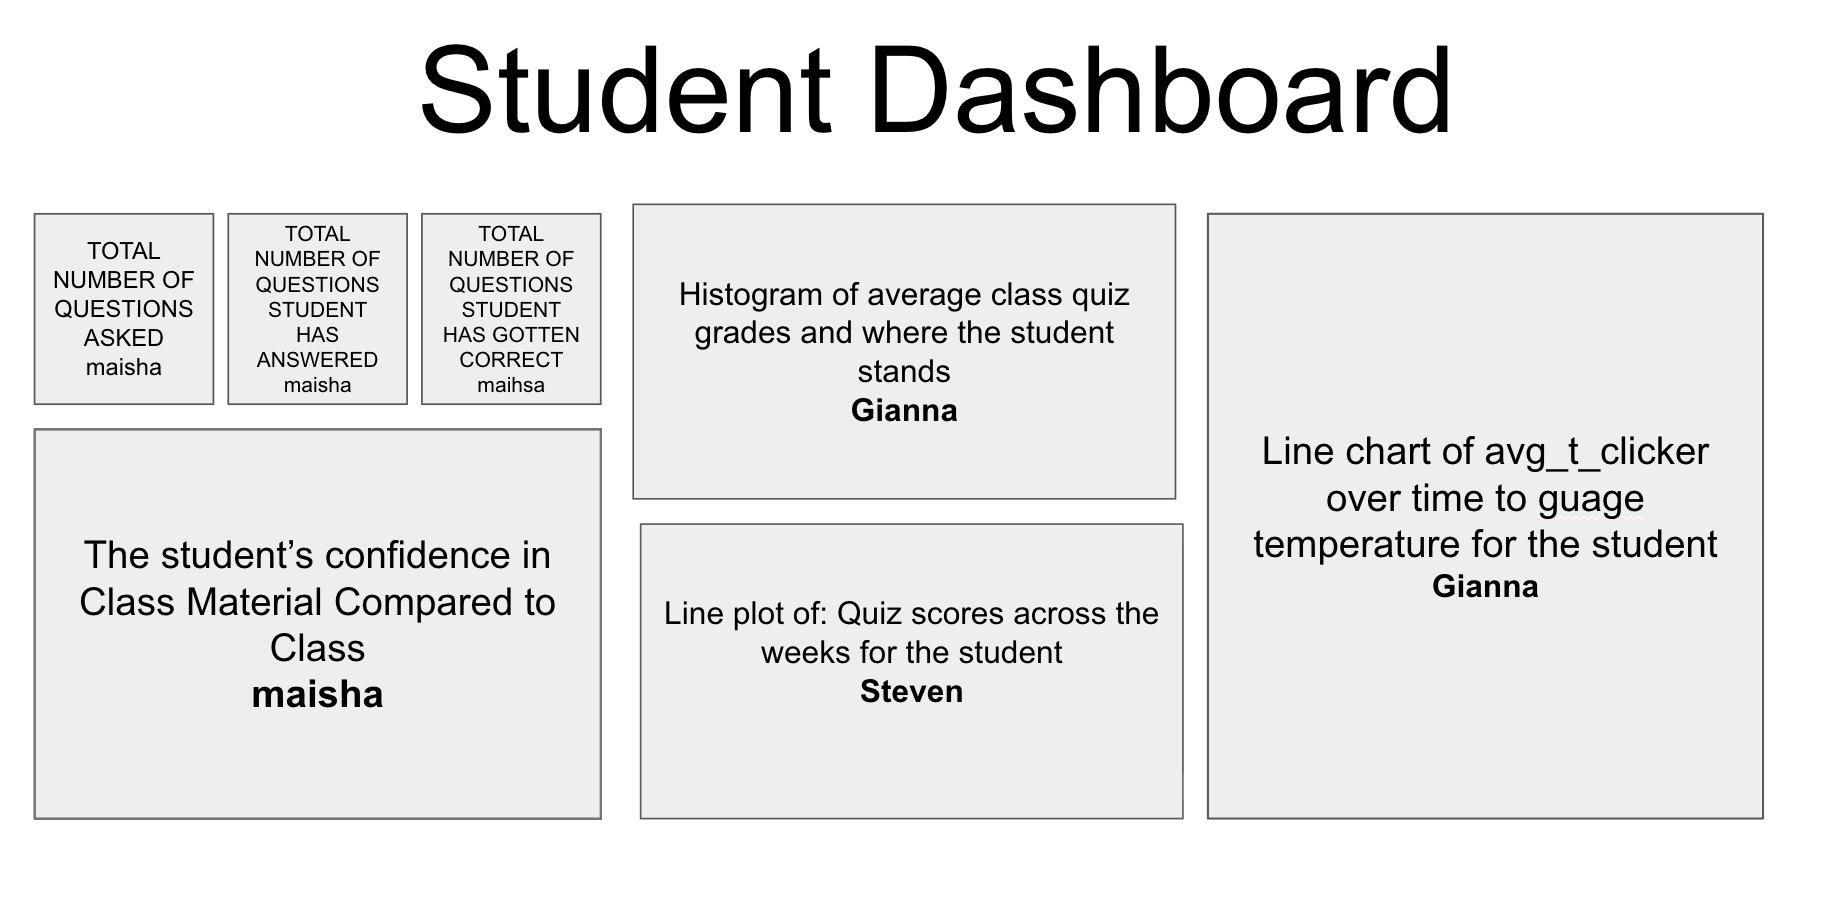
\includegraphics[keepaspectratio]{images/clipboard-3434643013.png}}

\pandocbounded{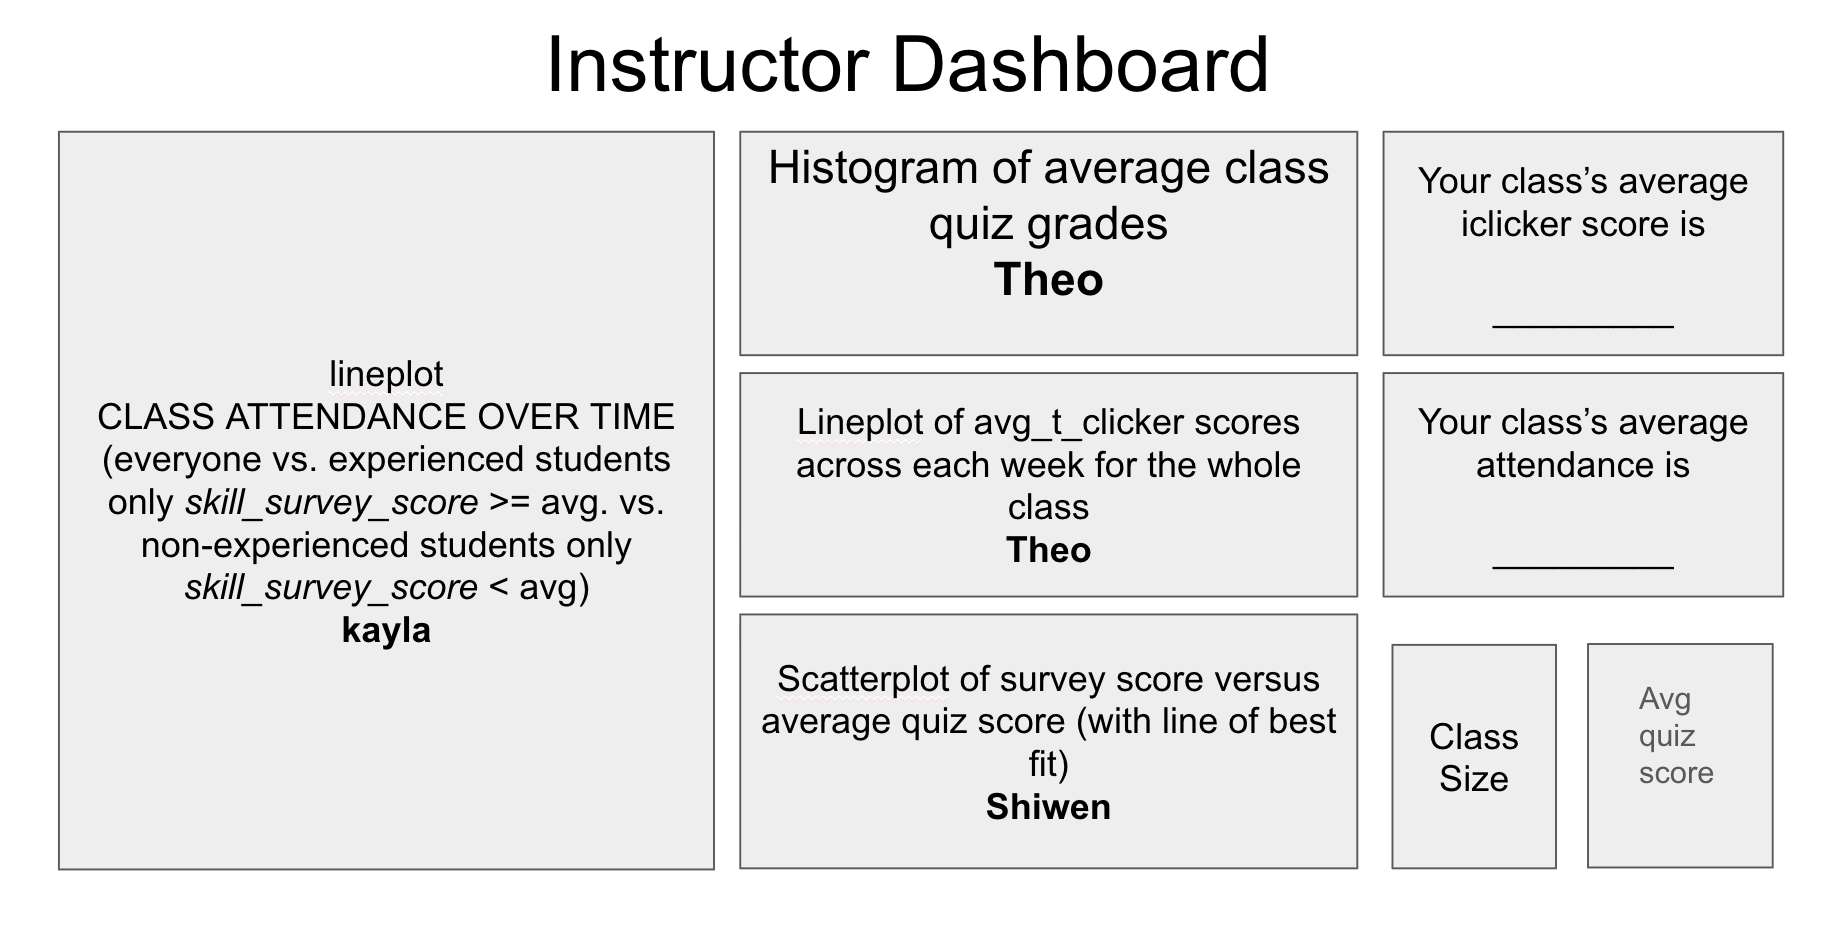
\includegraphics[keepaspectratio]{images/clipboard-349431012.png}}

\section{Part 2: Dashboard Wire-frame
Implementation}\label{part-2-dashboard-wire-frame-implementation}

This is where you generate the dashboard layout. You are given a very
basic wire frame example for the dashboard below. For more information
on how R Shiny Dashboards work, look at
\url{https://rstudio.github.io/shinydashboard/get_started.html} and
\url{https://rstudio.github.io/shinydashboard/structure.html}. You can
add different types of content into a \texttt{fuidRow()}. In the starter
code, there are 2 rows of content: the first has two little info boxes;
the second has two larger viz boxes. You can add more rows and change
what is in them as you wish. Follow the naming convention,
e.g.~\texttt{inst.info1} is the first info box for instructors.

Your team can split up the tasks. Some work on creating the UI (this
part), while others work on pre-processing the data and creating the
statistics and visualizations that will populate the UI (next part).

\textbf{Question 3:} Create the layout for the dashboard tabs. You can
have as many ``tabs'' as you like. Each tab is the content displayed
when the user clicks on one of the menu items (so it is the page
content). Here you are just specifying the wire frame i.e.~\textbf{what
goes where on the pages}, not what goes into it.

\begin{Shaded}
\begin{Highlighting}[]
\DocumentationTok{\#\#\#\#\#\#\#\#\#\#\#\#\#\#\#\#\#\#\#\#\#\#\#\#\#\#\#\#\#\#\#\#\#\#\#\#\#\#\#}
\DocumentationTok{\#\#\#\#\#\#\# }\RegionMarkerTok{BEGIN}\DocumentationTok{ INPUT: Question 3 \#\#\#\#\#\#\#}
\DocumentationTok{\#\#\#\#\#\#\#\#\#\#\#\#\#\#\#\#\#\#\#\#\#\#\#\#\#\#\#\#\#\#\#\#\#\#\#\#\#\#\#}
\CommentTok{\# Example of a tab (i.e. page)}
\NormalTok{instructor\_dash }\OtherTok{=} \FunctionTok{tabItem}\NormalTok{(}
    \AttributeTok{tabName =} \StringTok{"instructor"}\NormalTok{,}
    \FunctionTok{h2}\NormalTok{(}\StringTok{"Instructor Dashboard"}\NormalTok{),}
    
    \CommentTok{\# Dynamic infoBoxes}
   \CommentTok{\# fluidRow(}
   \CommentTok{\#   infoBoxOutput("attendance\_across\_lecture"),}
   \CommentTok{\#   infoBoxOutput("inst.info2")}
   \CommentTok{\# ),}
    \CommentTok{\# visualizations}
    \FunctionTok{fluidRow}\NormalTok{(}
      \FunctionTok{column}\NormalTok{(}
        \AttributeTok{width =} \DecValTok{8}\NormalTok{,}
        \FunctionTok{box}\NormalTok{(}
            \AttributeTok{title =} \StringTok{"Class Attendance by Lecture (by Skill Level)"}\NormalTok{,}
            \AttributeTok{width =} \DecValTok{12}\NormalTok{,}
            \FunctionTok{plotOutput}\NormalTok{(}\StringTok{"attendance\_across\_lecture"}\NormalTok{, }\AttributeTok{height =} \DecValTok{250}\NormalTok{)}
\NormalTok{        ),}
        \FunctionTok{box}\NormalTok{(}
            \AttributeTok{title =} \StringTok{"Avg Quiz Score per Student"}\NormalTok{,}
            \AttributeTok{width =} \DecValTok{12}\NormalTok{,}
            \FunctionTok{plotOutput}\NormalTok{(}\StringTok{"inst\_quiz\_hist"}\NormalTok{, }\AttributeTok{height =} \DecValTok{250}\NormalTok{)}
\NormalTok{        ),}
        \FunctionTok{box}\NormalTok{(}
            \AttributeTok{title =} \StringTok{"Class Temperature Across Lectures"}\NormalTok{,}
            \AttributeTok{width =} \DecValTok{12}\NormalTok{,}
            \FunctionTok{plotOutput}\NormalTok{(}\StringTok{"inst\_temp\_weekly"}\NormalTok{, }\AttributeTok{height =} \DecValTok{250}\NormalTok{)}
\NormalTok{        ),}
        \FunctionTok{box}\NormalTok{(}
            \AttributeTok{title =} \StringTok{"Survey Score vs Average Quiz Score"}\NormalTok{,}
            \AttributeTok{width =} \DecValTok{12}\NormalTok{,}
            \FunctionTok{plotOutput}\NormalTok{(}\StringTok{"survey\_vs\_quiz"}\NormalTok{, }\AttributeTok{height =} \DecValTok{250}\NormalTok{)}
\NormalTok{        )}
\NormalTok{    ),}
    \FunctionTok{column}\NormalTok{(}
    \AttributeTok{width =} \DecValTok{4}\NormalTok{,}
    \FunctionTok{infoBoxOutput}\NormalTok{(}\StringTok{"percent\_clicker\_correct"}\NormalTok{, }\AttributeTok{width =} \DecValTok{12}\NormalTok{),}
    \FunctionTok{infoBoxOutput}\NormalTok{(}\StringTok{"average\_quiz\_score"}\NormalTok{, }\AttributeTok{width =} \DecValTok{12}\NormalTok{),}
    \FunctionTok{infoBoxOutput}\NormalTok{(}\StringTok{"average\_attendance"}\NormalTok{, }\AttributeTok{width =} \DecValTok{12}\NormalTok{),}
    \FunctionTok{infoBoxOutput}\NormalTok{(}\StringTok{"class\_size"}\NormalTok{, }\AttributeTok{width =} \DecValTok{12}\NormalTok{)}
\NormalTok{    )}
\NormalTok{  )}
\NormalTok{)}

\CommentTok{\# Another empty tab}
\NormalTok{student\_dash }\OtherTok{=} \FunctionTok{tabItem}\NormalTok{(}
  \AttributeTok{tabName =} \StringTok{"student"}\NormalTok{,}
  \FunctionTok{h2}\NormalTok{(}\StringTok{"Student Dashboard"}\NormalTok{),}
  
  \FunctionTok{fluidRow}\NormalTok{(}
    \FunctionTok{selectInput}\NormalTok{(}\StringTok{"student\_id"}\NormalTok{, }\StringTok{"Select Student"}\NormalTok{,}
                \AttributeTok{choices =} \FunctionTok{sort}\NormalTok{(}\FunctionTok{unique}\NormalTok{(quiz}\SpecialCharTok{$}\NormalTok{STUDENT\_KEY)),}
                \AttributeTok{selected =} \DecValTok{105}\NormalTok{)}
\NormalTok{  ),}
  
  \FunctionTok{fluidRow}\NormalTok{(}
    \FunctionTok{box}\NormalTok{(}
      \AttributeTok{title =} \StringTok{"Your Average Quiz Score vs Class"}\NormalTok{,}
      \AttributeTok{width =} \DecValTok{12}\NormalTok{,}
      \FunctionTok{plotOutput}\NormalTok{(}\StringTok{"student\_hist"}\NormalTok{)}
\NormalTok{    )}
\NormalTok{  ),}
  
  \FunctionTok{fluidRow}\NormalTok{(}
    \FunctionTok{box}\NormalTok{(}
      \AttributeTok{title =} \StringTok{"Your Temperature (Engagement) Over Time"}\NormalTok{,}
      \AttributeTok{width =} \DecValTok{12}\NormalTok{,}
      \FunctionTok{plotOutput}\NormalTok{(}\StringTok{"student\_temp\_trend"}\NormalTok{)}
\NormalTok{    )}
\NormalTok{  ),}
  
  \FunctionTok{fluidRow}\NormalTok{(}
    \FunctionTok{box}\NormalTok{(}
      \AttributeTok{title =} \StringTok{"Your Confidence in Class Material Compared to Class"}\NormalTok{,}
      \AttributeTok{width =} \DecValTok{12}\NormalTok{,}
      \FunctionTok{plotOutput}\NormalTok{(}\StringTok{"temp\_clicker"}\NormalTok{)}
\NormalTok{    )}
\NormalTok{  ), }
  \FunctionTok{fluidRow}\NormalTok{(}
    \FunctionTok{box}\NormalTok{(}
      \AttributeTok{title =} \StringTok{"Your Quiz Scores Over Time"}\NormalTok{,}
      \AttributeTok{width =} \DecValTok{12}\NormalTok{,}
      \FunctionTok{plotOutput}\NormalTok{(}\StringTok{"student\_quiz\_trend"}\NormalTok{)}
\NormalTok{    )}
\NormalTok{  ),}
    \FunctionTok{fluidRow}\NormalTok{(}
      \FunctionTok{infoBoxOutput}\NormalTok{(}\StringTok{"total\_asked"}\NormalTok{, }\AttributeTok{width =} \DecValTok{4}\NormalTok{),}
      \FunctionTok{infoBoxOutput}\NormalTok{(}\StringTok{"total\_answered"}\NormalTok{, }\AttributeTok{width =} \DecValTok{4}\NormalTok{),}
      \FunctionTok{infoBoxOutput}\NormalTok{(}\StringTok{"total\_correct"}\NormalTok{, }\AttributeTok{width =} \DecValTok{4}\NormalTok{)}
\NormalTok{  )}
\NormalTok{)}
\DocumentationTok{\#\#\#\#\#\#\#\#\#\#\#\#\#\#\#\#\#\#\#\#\#\#\#\#\#\#\#\#\#\#\#\#\#\#\#\#\#\#\#}
\DocumentationTok{\#\#\#\#\#\#\#\#\#\#\#\#\#\#\#\#\#\#\#\#\#\#\#\#\#\#\#\#\#\#\#\#\#\#\#\#\#\#\#}
\end{Highlighting}
\end{Shaded}

\section{Part 3: Data Pre-processing}\label{part-3-data-pre-processing}

Get the data ready for use in the dashboard. Before the next stage, you
want to have the data ready in the right format for simple computations
and plotting. To do this effectively, you need to know by now what you
want to display in each dashboard. However, this is also an iterative
process. Once you have completed a first iteration of the design, you
can come back to this step and add further pre-processing for more
visualizations you like to add. This step is also an opportunity to
better understand the structure of the datasets.

The instructor dashboard should show information for all students. The
student dashboard is typically focused on an individual student. You can
either pick a student (at random or intentionally) and use them as the
``reference student'' for the student dashboard. Or, a bit more
ambitious but also more rewarding to try out, you can create an
interactive dashboard in which you select the student and then the
dashboard updates to show the information for that student. I would
recommend you start with the simpler version and get that to work before
you try to make it dynamic.

Use the space below to be ready for your information visualizations in
the dashboards.

\begin{Shaded}
\begin{Highlighting}[]
\DocumentationTok{\#\#\#\#\#\#\#\#\#\#\#\#\#\#\#\#\#\#\#\#\#\#\#\#\#\#\#\#\#\#\#\#\#\#\#\#\#\#\#}
\DocumentationTok{\#\#\#\#\#\#\# }\RegionMarkerTok{BEGIN}\DocumentationTok{ INPUT             \#\#\#\#\#\#\#}
\DocumentationTok{\#\#\#\#\#\#\#\#\#\#\#\#\#\#\#\#\#\#\#\#\#\#\#\#\#\#\#\#\#\#\#\#\#\#\#\#\#\#\#}

\CommentTok{\# combine quiz and experience datasets by STUDENT\_KEY and YEAR}
\NormalTok{df }\OtherTok{\textless{}{-}} \FunctionTok{left\_join}\NormalTok{(quiz, experience, }\AttributeTok{by =} \FunctionTok{c}\NormalTok{(}\StringTok{"STUDENT\_KEY"}\NormalTok{, }\StringTok{"YEAR"}\NormalTok{))}
\FunctionTok{head}\NormalTok{(df)}
\end{Highlighting}
\end{Shaded}

\begin{verbatim}
##   ACAD_DATE_KEY STUDENT_KEY YEAR SESSION_NUMBER QUIZ_NUMBER ATTENDED
## 1      20170905         105 2017              8           3        1
## 2      20170912          32 2017             10           4        1
## 3      20170825          68 2017              5           1        1
## 4      20180906         103 2018              5           4        1
## 5      20170824          68 2017              2           1        1
## 6      20170914          12 2017             12           4        1
##   TOTAL_POSSIBLE_CLICKER TOTAL_COMPLETED_CLICKER COMPLETED_Q_CLICKER
## 1                      5                       4                   4
## 2                      2                       1                   1
## 3                      1                       1                   0
## 4                      6                       3                   1
## 5                      3                       2                   3
## 6                      4                       4                   2
##   CORRECT_Q_CLICKER COMPLETED_T_CLICKER AVG_T_CLICKER QUIZ_SCORE  PROG
## 1                 3                   1           4.0         20  GRAD
## 2                 0                   0           0.0         20 UGRAD
## 3                 0                   1           2.0         18  GRAD
## 4                 0                   2           3.0         17  GRAD
## 5                 0                   0           0.0         18  GRAD
## 6                 0                   2           2.5         17  GRAD
##   DATABASE_SCORE SQL_SCORE PROGRAMING_SCORE STORED_PROC_SCORE ETL_SCORE
## 1              1         1                3                 0         1
## 2             NA        NA               NA                NA        NA
## 3              1         1                2                 1         1
## 4              3         4                4                 3         4
## 5              1         1                2                 1         1
## 6             NA        NA               NA                NA        NA
##   DATA_VIS_SCORE REQUIREMENT_GATHER_SCORE SKILL_SURVEY_SCORE
## 1              0                        0                  6
## 2             NA                       NA                 NA
## 3              0                        0                  6
## 4              2                        0                 20
## 5              0                        0                  6
## 6             NA                       NA                 NA
\end{verbatim}

\begin{Shaded}
\begin{Highlighting}[]
\CommentTok{\# creates dataframe grouped by lecture}
\CommentTok{\# for some lectures, there are multiple iClicker sessions}
\CommentTok{\# the grouping combines the sessions into one per lecture}
\NormalTok{df\_by\_lecture }\OtherTok{\textless{}{-}}\NormalTok{ df }\SpecialCharTok{\%\textgreater{}\%}
  \FunctionTok{group\_by}\NormalTok{(STUDENT\_KEY, }
\NormalTok{           ACAD\_DATE\_KEY, }
\NormalTok{           YEAR, }
\NormalTok{           QUIZ\_NUMBER,}
\NormalTok{           ATTENDED, }
\NormalTok{           PROG,}
\NormalTok{           DATABASE\_SCORE, }
\NormalTok{           SQL\_SCORE, }
\NormalTok{           PROGRAMING\_SCORE,}
\NormalTok{           STORED\_PROC\_SCORE,}
\NormalTok{           ETL\_SCORE,}
\NormalTok{           DATA\_VIS\_SCORE,}
\NormalTok{           REQUIREMENT\_GATHER\_SCORE,}
\NormalTok{           SKILL\_SURVEY\_SCORE) }\SpecialCharTok{\%\textgreater{}\%}
  \FunctionTok{summarise}\NormalTok{(}\AttributeTok{SESSION\_NUMBER =} \FunctionTok{min}\NormalTok{(SESSION\_NUMBER),}
            \AttributeTok{TOTAL\_POSSIBLE\_CLICKER =} \FunctionTok{sum}\NormalTok{(TOTAL\_POSSIBLE\_CLICKER),}
            \AttributeTok{TOTAL\_COMPLETED\_CLICKER =} \FunctionTok{sum}\NormalTok{(TOTAL\_COMPLETED\_CLICKER),}
            \AttributeTok{COMPLETED\_Q\_CLICKER =} \FunctionTok{sum}\NormalTok{(COMPLETED\_Q\_CLICKER),}
            \AttributeTok{CORRECT\_Q\_CLICKER =} \FunctionTok{sum}\NormalTok{(CORRECT\_Q\_CLICKER),}
            \AttributeTok{COMPLETED\_T\_CLICKER =} \FunctionTok{sum}\NormalTok{(COMPLETED\_T\_CLICKER),}
            \AttributeTok{AVG\_T\_CLICKER =} \FunctionTok{mean}\NormalTok{(AVG\_T\_CLICKER),}
            \AttributeTok{QUIZ\_SCORE =} \FunctionTok{mean}\NormalTok{(QUIZ\_SCORE, }\AttributeTok{na.rm =} \ConstantTok{TRUE}\NormalTok{)) }\SpecialCharTok{\%\textgreater{}\%}
  \FunctionTok{arrange}\NormalTok{(STUDENT\_KEY, ACAD\_DATE\_KEY)}
\end{Highlighting}
\end{Shaded}

\begin{verbatim}
## `summarise()` has grouped output by 'STUDENT_KEY', 'ACAD_DATE_KEY', 'YEAR',
## 'QUIZ_NUMBER', 'ATTENDED', 'PROG', 'DATABASE_SCORE', 'SQL_SCORE',
## 'PROGRAMING_SCORE', 'STORED_PROC_SCORE', 'ETL_SCORE', 'DATA_VIS_SCORE',
## 'REQUIREMENT_GATHER_SCORE'. You can override using the `.groups` argument.
\end{verbatim}

\begin{Shaded}
\begin{Highlighting}[]
\CommentTok{\# since we combined sessions where there were multiple per lecture,}
\CommentTok{\# let\textquotesingle{}s add a field to indicate each lecture by number}
\CommentTok{\# LECTURE\_NUMBER}
\NormalTok{df\_by\_lecture }\OtherTok{\textless{}{-}}\NormalTok{ df\_by\_lecture }\SpecialCharTok{\%\textgreater{}\%}
  \FunctionTok{group\_by}\NormalTok{(STUDENT\_KEY) }\SpecialCharTok{\%\textgreater{}\%}
  \FunctionTok{arrange}\NormalTok{(SESSION\_NUMBER, }\AttributeTok{.by\_group =} \ConstantTok{TRUE}\NormalTok{) }\SpecialCharTok{\%\textgreater{}\%}
  \FunctionTok{mutate}\NormalTok{(}\AttributeTok{LECTURE\_NUMBER =} \FunctionTok{row\_number}\NormalTok{()) }\SpecialCharTok{\%\textgreater{}\%}
  \FunctionTok{ungroup}\NormalTok{()}

\FunctionTok{head}\NormalTok{(df\_by\_lecture)}
\end{Highlighting}
\end{Shaded}

\begin{verbatim}
## # A tibble: 6 x 23
##   STUDENT_KEY ACAD_DATE_KEY  YEAR QUIZ_NUMBER ATTENDED PROG  DATABASE_SCORE
##         <int>         <int> <int>       <int>    <int> <chr>          <int>
## 1           1      20180828  2018           1        1 UGRAD              1
## 2           1      20180830  2018           2        1 UGRAD              1
## 3           1      20180904  2018           3        1 UGRAD              1
## 4           1      20180906  2018           4        1 UGRAD              1
## 5           1      20180911  2018           5        0 UGRAD              1
## 6           1      20180918  2018           6        1 UGRAD              1
## # i 16 more variables: SQL_SCORE <int>, PROGRAMING_SCORE <int>,
## #   STORED_PROC_SCORE <int>, ETL_SCORE <int>, DATA_VIS_SCORE <int>,
## #   REQUIREMENT_GATHER_SCORE <int>, SKILL_SURVEY_SCORE <int>,
## #   SESSION_NUMBER <int>, TOTAL_POSSIBLE_CLICKER <int>,
## #   TOTAL_COMPLETED_CLICKER <int>, COMPLETED_Q_CLICKER <int>,
## #   CORRECT_Q_CLICKER <int>, COMPLETED_T_CLICKER <int>, AVG_T_CLICKER <dbl>,
## #   QUIZ_SCORE <dbl>, LECTURE_NUMBER <int>
\end{verbatim}

\begin{Shaded}
\begin{Highlighting}[]
\DocumentationTok{\#\#\#\#\#\#\#\#\#\#\#\#\#\#\#\#\#\#\#\#\#\#\#\#\#\#\#\#\#\#\#\#\#\#\#\#\#\#\#}
\DocumentationTok{\#\#\#\#\#\#\#\#\#\#\#\#\#\#\#\#\#\#\#\#\#\#\#\#\#\#\#\#\#\#\#\#\#\#\#\#\#\#\#}
\end{Highlighting}
\end{Shaded}

\section{Part 4: Prepare All Data
Visualizations}\label{part-4-prepare-all-data-visualizations}

This is where you create the content for the wire frames you created
above. Again, you can refer to the examples and documentation in
\url{https://rstudio.github.io/shinydashboard/get_started.html} and
\url{https://rstudio.github.io/shinydashboard/structure.html} for
guidance. You can also find many examples online just by searching with
Google.

\textbf{Question 4:} For each of the pieces of content you planned for
in the wire frames above, generate the relevant content. You need to
assign them all to the \texttt{output} variable by referencing the name
of the wire frame element you chose above like this
\texttt{output\$name.of.element}.

\begin{Shaded}
\begin{Highlighting}[]
\NormalTok{server }\OtherTok{=} \ControlFlowTok{function}\NormalTok{(input, output) \{}
    
\DocumentationTok{\#\#\#\#\#\#\#\#\#\#\#\#\#\#\#\#\#\#\#\#\#\#\#\#\#\#\#\#\#\#\#\#\#\#\#\#\#\#\#}
\DocumentationTok{\#\#\#\#\#\#\# }\RegionMarkerTok{BEGIN}\DocumentationTok{ INPUT: Question 4 \#\#\#\#\#\#\#}
\DocumentationTok{\#\#\#\#\#\#\#\#\#\#\#\#\#\#\#\#\#\#\#\#\#\#\#\#\#\#\#\#\#\#\#\#\#\#\#\#\#\#\#}
    
\NormalTok{    output}\SpecialCharTok{$}\NormalTok{inst.info1 }\OtherTok{=} \FunctionTok{renderInfoBox}\NormalTok{(\{}
        \FunctionTok{infoBox}\NormalTok{(}\StringTok{"Students total"}\NormalTok{, }
                \FunctionTok{length}\NormalTok{(}\FunctionTok{unique}\NormalTok{(quiz}\SpecialCharTok{$}\NormalTok{STUDENT\_KEY)), }
                \AttributeTok{icon =} \FunctionTok{icon}\NormalTok{(}\StringTok{"list"}\NormalTok{), }\AttributeTok{color =} \StringTok{"purple"}\NormalTok{)}
\NormalTok{    \})}
    
\NormalTok{    output}\SpecialCharTok{$}\NormalTok{inst.info2 }\OtherTok{=} \FunctionTok{renderInfoBox}\NormalTok{(\{}
        \FunctionTok{infoBox}\NormalTok{(}\StringTok{"Attendance"}\NormalTok{,}
                \FunctionTok{paste0}\NormalTok{(}\FunctionTok{round}\NormalTok{(}\DecValTok{100} \SpecialCharTok{*} \FunctionTok{mean}\NormalTok{(quiz}\SpecialCharTok{$}\NormalTok{ATTENDED)), }\StringTok{"\%"}\NormalTok{), }
                \AttributeTok{icon =} \FunctionTok{icon}\NormalTok{(}\StringTok{"list"}\NormalTok{), }\AttributeTok{color =} \StringTok{"yellow"}\NormalTok{)}
\NormalTok{    \})}
    
\NormalTok{    output}\SpecialCharTok{$}\NormalTok{inst.plot1 }\OtherTok{=} \FunctionTok{renderPlot}\NormalTok{(\{}
        \FunctionTok{hist}\NormalTok{(quiz}\SpecialCharTok{$}\NormalTok{QUIZ\_SCORE)}
\NormalTok{    \})}
    
\NormalTok{    output}\SpecialCharTok{$}\NormalTok{student\_temp\_trend }\OtherTok{=} \FunctionTok{renderPlot}\NormalTok{(\{}
  
\NormalTok{    student\_data }\OtherTok{\textless{}{-}}\NormalTok{ df\_by\_lecture }\SpecialCharTok{\%\textgreater{}\%}
    \FunctionTok{filter}\NormalTok{(STUDENT\_KEY }\SpecialCharTok{==}\NormalTok{ input}\SpecialCharTok{$}\NormalTok{student\_id)}
  
    \FunctionTok{ggplot}\NormalTok{(student\_data, }\FunctionTok{aes}\NormalTok{(}\AttributeTok{x =}\NormalTok{ LECTURE\_NUMBER, }\AttributeTok{y =}\NormalTok{ AVG\_T\_CLICKER)) }\SpecialCharTok{+}
    \FunctionTok{geom\_line}\NormalTok{(}\AttributeTok{color =} \StringTok{"\#2C7FB8"}\NormalTok{, }\AttributeTok{size =} \FloatTok{1.5}\NormalTok{) }\SpecialCharTok{+}
    \FunctionTok{geom\_point}\NormalTok{(}\AttributeTok{color =} \StringTok{"\#2C7FB8"}\NormalTok{, }\AttributeTok{size =} \DecValTok{2}\NormalTok{) }\SpecialCharTok{+}
    
    \FunctionTok{labs}\NormalTok{(}
      \AttributeTok{title =} \FunctionTok{paste}\NormalTok{(}\StringTok{"Temperature Trend for Student"}\NormalTok{, input}\SpecialCharTok{$}\NormalTok{student\_id),}
      \AttributeTok{x =} \StringTok{"Lecture Number"}\NormalTok{,}
      \AttributeTok{y =} \StringTok{"Average Temperature (0–5)"}
\NormalTok{    ) }\SpecialCharTok{+}
    
    \FunctionTok{ylim}\NormalTok{(}\DecValTok{0}\NormalTok{, }\DecValTok{5}\NormalTok{) }\SpecialCharTok{+}
    \FunctionTok{theme\_classic}\NormalTok{()}
\NormalTok{    \})}
    
\NormalTok{    output}\SpecialCharTok{$}\NormalTok{student\_quiz\_trend }\OtherTok{=} \FunctionTok{renderPlot}\NormalTok{(\{}
\NormalTok{        student\_quiz }\OtherTok{\textless{}{-}}\NormalTok{ df\_by\_lecture }\SpecialCharTok{\%\textgreater{}\%}
          \FunctionTok{filter}\NormalTok{(STUDENT\_KEY }\SpecialCharTok{==}\NormalTok{ input}\SpecialCharTok{$}\NormalTok{student\_id, }\SpecialCharTok{!}\FunctionTok{is.na}\NormalTok{(QUIZ\_SCORE)) }\SpecialCharTok{\%\textgreater{}\%}
          \FunctionTok{group\_by}\NormalTok{(QUIZ\_NUMBER) }\SpecialCharTok{\%\textgreater{}\%}
          \FunctionTok{summarise}\NormalTok{(}\AttributeTok{quiz\_score =} \FunctionTok{first}\NormalTok{(QUIZ\_SCORE), }\AttributeTok{.groups =} \StringTok{"drop"}\NormalTok{)}
    
        \FunctionTok{ggplot}\NormalTok{(student\_quiz, }\FunctionTok{aes}\NormalTok{(}\AttributeTok{x =}\NormalTok{ QUIZ\_NUMBER, }\AttributeTok{y =}\NormalTok{ quiz\_score)) }\SpecialCharTok{+}
          \FunctionTok{geom\_line}\NormalTok{(}\AttributeTok{color =} \StringTok{"\#2C7FB8"}\NormalTok{, }\AttributeTok{linewidth =} \FloatTok{1.5}\NormalTok{) }\SpecialCharTok{+}
          \FunctionTok{geom\_point}\NormalTok{(}\AttributeTok{color =} \StringTok{"\#2C7FB8"}\NormalTok{, }\AttributeTok{size =} \DecValTok{3}\NormalTok{) }\SpecialCharTok{+}
          \FunctionTok{scale\_y\_continuous}\NormalTok{(}\AttributeTok{limits =} \FunctionTok{c}\NormalTok{(}\DecValTok{0}\NormalTok{, }\DecValTok{20}\NormalTok{)) }\SpecialCharTok{+}
          \FunctionTok{scale\_x\_continuous}\NormalTok{(}\AttributeTok{breaks =} \DecValTok{1}\SpecialCharTok{:}\DecValTok{10}\NormalTok{) }\SpecialCharTok{+}
          \FunctionTok{labs}\NormalTok{(}
            \AttributeTok{title =} \FunctionTok{paste}\NormalTok{(}\StringTok{"Quiz Score Trend for Student"}\NormalTok{, input}\SpecialCharTok{$}\NormalTok{student\_id),}
            \AttributeTok{x =} \StringTok{"Quiz Number"}\NormalTok{,}
            \AttributeTok{y =} \StringTok{"Quiz Score (out of 20)"}
\NormalTok{          ) }\SpecialCharTok{+}
          \FunctionTok{theme\_classic}\NormalTok{()}
\NormalTok{    \})}
    
\NormalTok{    output}\SpecialCharTok{$}\NormalTok{student\_hist }\OtherTok{=} \FunctionTok{renderPlot}\NormalTok{(\{}
  
    \CommentTok{\# average quiz score per student}
\NormalTok{    avg\_quiz\_by\_student }\OtherTok{\textless{}{-}}\NormalTok{ df\_by\_lecture }\SpecialCharTok{\%\textgreater{}\%}
    \FunctionTok{group\_by}\NormalTok{(STUDENT\_KEY) }\SpecialCharTok{\%\textgreater{}\%}
    \FunctionTok{summarise}\NormalTok{(}\AttributeTok{avg\_quiz =} \FunctionTok{mean}\NormalTok{(QUIZ\_SCORE, }\AttributeTok{na.rm =} \ConstantTok{TRUE}\NormalTok{))}
  
    \CommentTok{\# selected student value}
\NormalTok{    student\_avg }\OtherTok{\textless{}{-}}\NormalTok{ avg\_quiz\_by\_student }\SpecialCharTok{\%\textgreater{}\%}
    \FunctionTok{filter}\NormalTok{(STUDENT\_KEY }\SpecialCharTok{==}\NormalTok{ input}\SpecialCharTok{$}\NormalTok{student\_id) }\SpecialCharTok{\%\textgreater{}\%}
    \FunctionTok{pull}\NormalTok{(avg\_quiz)}
  
    \CommentTok{\# class average (optional but recommended)}
\NormalTok{    class\_avg }\OtherTok{\textless{}{-}} \FunctionTok{mean}\NormalTok{(avg\_quiz\_by\_student}\SpecialCharTok{$}\NormalTok{avg\_quiz, }\AttributeTok{na.rm =} \ConstantTok{TRUE}\NormalTok{)}
  
    \FunctionTok{ggplot}\NormalTok{(avg\_quiz\_by\_student, }\FunctionTok{aes}\NormalTok{(}\AttributeTok{x =}\NormalTok{ avg\_quiz)) }\SpecialCharTok{+}
    \FunctionTok{geom\_histogram}\NormalTok{(}\AttributeTok{binwidth =} \DecValTok{4}\NormalTok{, }\AttributeTok{fill =} \StringTok{"\#BCD8EC"}\NormalTok{, }\AttributeTok{color =} \StringTok{"black"}\NormalTok{) }\SpecialCharTok{+}
    
    \CommentTok{\# student line}
    \FunctionTok{geom\_vline}\NormalTok{(}\AttributeTok{xintercept =}\NormalTok{ student\_avg,}
               \AttributeTok{color =} \StringTok{"blue"}\NormalTok{,}
               \AttributeTok{size =} \FloatTok{1.5}\NormalTok{) }\SpecialCharTok{+}
    
    \CommentTok{\# class average line}
    \FunctionTok{geom\_vline}\NormalTok{(}\AttributeTok{xintercept =}\NormalTok{ class\_avg,}
               \AttributeTok{color =} \StringTok{"red"}\NormalTok{,}
               \AttributeTok{linetype =} \StringTok{"dashed"}\NormalTok{,}
               \AttributeTok{size =} \FloatTok{1.2}\NormalTok{) }\SpecialCharTok{+}
    
    \FunctionTok{labs}\NormalTok{(}
      \AttributeTok{title =} \StringTok{"Distribution of Average Quiz Scores"}\NormalTok{,}
      \AttributeTok{x =} \StringTok{"Average Quiz Score"}\NormalTok{,}
      \AttributeTok{y =} \StringTok{"Number of Students"}
\NormalTok{    ) }\SpecialCharTok{+}
    
    \FunctionTok{annotate}\NormalTok{(}\StringTok{"text"}\NormalTok{,}
             \AttributeTok{x =}\NormalTok{ student\_avg,}
             \AttributeTok{y =} \ConstantTok{Inf}\NormalTok{,}
             \AttributeTok{label =} \FunctionTok{paste}\NormalTok{(}\StringTok{"You ("}\NormalTok{, input}\SpecialCharTok{$}\NormalTok{student\_id, }\StringTok{")"}\NormalTok{, }\AttributeTok{sep =} \StringTok{""}\NormalTok{),}
             \AttributeTok{vjust =} \SpecialCharTok{{-}}\FloatTok{0.5}\NormalTok{,}
             \AttributeTok{color =} \StringTok{\textquotesingle{}\#FFBCE1\textquotesingle{}}\NormalTok{) }\SpecialCharTok{+}
    
    \FunctionTok{theme\_classic}\NormalTok{()}
\NormalTok{    \})}
\NormalTok{    output}\SpecialCharTok{$}\NormalTok{inst\_quiz\_hist }\OtherTok{=} \FunctionTok{renderPlot}\NormalTok{(\{}
\NormalTok{        student\_avg\_quiz }\OtherTok{\textless{}{-}}\NormalTok{ df\_by\_lecture }\SpecialCharTok{\%\textgreater{}\%}
          \FunctionTok{filter}\NormalTok{(}\SpecialCharTok{!}\FunctionTok{is.na}\NormalTok{(QUIZ\_SCORE)) }\SpecialCharTok{\%\textgreater{}\%}
          \FunctionTok{group\_by}\NormalTok{(STUDENT\_KEY) }\SpecialCharTok{\%\textgreater{}\%}
          \FunctionTok{summarize}\NormalTok{(}\AttributeTok{avg\_quiz =} \FunctionTok{mean}\NormalTok{(QUIZ\_SCORE, }\AttributeTok{na.rm =} \ConstantTok{TRUE}\NormalTok{), }\AttributeTok{.groups =} \StringTok{"drop"}\NormalTok{)}
    
        \FunctionTok{ggplot}\NormalTok{(student\_avg\_quiz, }\FunctionTok{aes}\NormalTok{(}\AttributeTok{x =}\NormalTok{ avg\_quiz)) }\SpecialCharTok{+}
          \FunctionTok{geom\_histogram}\NormalTok{(}\AttributeTok{binwidth =} \DecValTok{1}\NormalTok{, }\AttributeTok{fill =} \StringTok{"\#BCD8EC"}\NormalTok{, }\AttributeTok{color =} \StringTok{"white"}\NormalTok{) }\SpecialCharTok{+}
          \FunctionTok{labs}\NormalTok{(}
            \AttributeTok{title =} \StringTok{"Distribution of Average Quiz Scores per Student"}\NormalTok{,}
            \AttributeTok{subtitle =} \FunctionTok{paste0}\NormalTok{(}\StringTok{"n = "}\NormalTok{, }\FunctionTok{nrow}\NormalTok{(student\_avg\_quiz), }\StringTok{" students"}\NormalTok{),}
            \AttributeTok{x =} \StringTok{"Average Quiz Score (out of 20)"}\NormalTok{,}
            \AttributeTok{y =} \StringTok{"Number of Students"}
\NormalTok{          ) }\SpecialCharTok{+}
          \FunctionTok{theme\_classic}\NormalTok{()}
\NormalTok{    \})}
    
\NormalTok{    output}\SpecialCharTok{$}\NormalTok{inst\_temp\_weekly }\OtherTok{=} \FunctionTok{renderPlot}\NormalTok{(\{}
\NormalTok{        weekly\_temp }\OtherTok{\textless{}{-}}\NormalTok{ df\_by\_lecture }\SpecialCharTok{\%\textgreater{}\%}
          \FunctionTok{filter}\NormalTok{(}\SpecialCharTok{!}\FunctionTok{is.na}\NormalTok{(AVG\_T\_CLICKER), LECTURE\_NUMBER }\SpecialCharTok{\textless{}} \DecValTok{21}\NormalTok{) }\SpecialCharTok{\%\textgreater{}\%}
          \FunctionTok{group\_by}\NormalTok{(LECTURE\_NUMBER) }\SpecialCharTok{\%\textgreater{}\%}
          \FunctionTok{summarize}\NormalTok{(}\AttributeTok{class\_avg\_t =} \FunctionTok{mean}\NormalTok{(AVG\_T\_CLICKER, }\AttributeTok{na.rm =} \ConstantTok{TRUE}\NormalTok{), }\AttributeTok{.groups =} \StringTok{"drop"}\NormalTok{)}
    
        \FunctionTok{ggplot}\NormalTok{(weekly\_temp, }\FunctionTok{aes}\NormalTok{(}\AttributeTok{x =}\NormalTok{ LECTURE\_NUMBER, }\AttributeTok{y =}\NormalTok{ class\_avg\_t)) }\SpecialCharTok{+}
          \FunctionTok{geom\_line}\NormalTok{(}\AttributeTok{color =} \StringTok{"\#2C7FB8"}\NormalTok{, }\AttributeTok{linewidth =} \DecValTok{1}\NormalTok{) }\SpecialCharTok{+}
          \FunctionTok{geom\_point}\NormalTok{(}\AttributeTok{color =} \StringTok{"\#2C7FB8"}\NormalTok{, }\AttributeTok{size =} \DecValTok{2}\NormalTok{) }\SpecialCharTok{+}
          \FunctionTok{scale\_y\_continuous}\NormalTok{(}\AttributeTok{limits =} \FunctionTok{c}\NormalTok{(}\DecValTok{0}\NormalTok{, }\DecValTok{5}\NormalTok{)) }\SpecialCharTok{+}
          \FunctionTok{scale\_x\_continuous}\NormalTok{(}\AttributeTok{breaks =} \FunctionTok{seq}\NormalTok{(}\DecValTok{1}\NormalTok{, }\DecValTok{20}\NormalTok{, }\AttributeTok{by =} \DecValTok{1}\NormalTok{)) }\SpecialCharTok{+}
          \FunctionTok{labs}\NormalTok{(}
            \AttributeTok{title =} \StringTok{"Class Average Temperature by Lecture"}\NormalTok{,}
            \AttributeTok{subtitle =} \StringTok{"0 = negative, 5 = positive"}\NormalTok{,}
            \AttributeTok{x =} \StringTok{"Lecture Number"}\NormalTok{,}
            \AttributeTok{y =} \StringTok{"Class Average Temperature"}
\NormalTok{          ) }\SpecialCharTok{+}
          \FunctionTok{theme\_classic}\NormalTok{()}
\NormalTok{    \})}
    
\NormalTok{    output}\SpecialCharTok{$}\NormalTok{attendance\_across\_lecture }\OtherTok{=} \FunctionTok{renderPlot}\NormalTok{(\{}
    
      \CommentTok{\# to compare class attendance per lecture,}
      \CommentTok{\# we need to group the data by lecture}
\NormalTok{      attendance\_per\_lecture }\OtherTok{\textless{}{-}}\NormalTok{ df\_by\_lecture }\SpecialCharTok{\%\textgreater{}\%}
        \FunctionTok{group\_by}\NormalTok{(LECTURE\_NUMBER) }\SpecialCharTok{\%\textgreater{}\%}
        \FunctionTok{summarise}\NormalTok{(}\AttributeTok{TOTAL\_AVG\_ATTENDANCE =} \FunctionTok{mean}\NormalTok{(ATTENDED))}
      
\NormalTok{      avg\_skill\_survery\_score }\OtherTok{\textless{}{-}} \FunctionTok{mean}\NormalTok{(df\_by\_lecture}\SpecialCharTok{$}\NormalTok{SKILL\_SURVEY\_SCORE, }\AttributeTok{na.rm =} \ConstantTok{TRUE}\NormalTok{)}
      
\NormalTok{      less\_skilled\_attendance\_per\_lecture }\OtherTok{\textless{}{-}}\NormalTok{ df\_by\_lecture }\SpecialCharTok{\%\textgreater{}\%}
        \FunctionTok{filter}\NormalTok{(SKILL\_SURVEY\_SCORE }\SpecialCharTok{\textless{}}\NormalTok{ avg\_skill\_survery\_score) }\SpecialCharTok{\%\textgreater{}\%}
        \FunctionTok{group\_by}\NormalTok{(LECTURE\_NUMBER) }\SpecialCharTok{\%\textgreater{}\%}
        \FunctionTok{summarise}\NormalTok{(}\AttributeTok{LESS\_SKILLED\_AVG\_ATTENDANCE =} \FunctionTok{mean}\NormalTok{(ATTENDED))}
      
\NormalTok{      more\_skilled\_attendance\_per\_lecture }\OtherTok{\textless{}{-}}\NormalTok{ df\_by\_lecture }\SpecialCharTok{\%\textgreater{}\%}
        \FunctionTok{filter}\NormalTok{(SKILL\_SURVEY\_SCORE }\SpecialCharTok{\textgreater{}=}\NormalTok{ avg\_skill\_survery\_score) }\SpecialCharTok{\%\textgreater{}\%}
        \FunctionTok{group\_by}\NormalTok{(LECTURE\_NUMBER) }\SpecialCharTok{\%\textgreater{}\%}
        \FunctionTok{summarise}\NormalTok{(}\AttributeTok{MORE\_SKILLED\_AVG\_ATTENDANCE =} \FunctionTok{mean}\NormalTok{(ATTENDED))}
      
\NormalTok{      attendance\_per\_lecture }\OtherTok{\textless{}{-}}\NormalTok{ attendance\_per\_lecture }\SpecialCharTok{\%\textgreater{}\%} 
        \FunctionTok{inner\_join}\NormalTok{(less\_skilled\_attendance\_per\_lecture) }\SpecialCharTok{\%\textgreater{}\%}
        \FunctionTok{inner\_join}\NormalTok{(more\_skilled\_attendance\_per\_lecture)}
      
\NormalTok{      attendance\_per\_lecture }\OtherTok{\textless{}{-}}\NormalTok{ attendance\_per\_lecture }\SpecialCharTok{\%\textgreater{}\%}
        \FunctionTok{pivot\_longer}\NormalTok{(}\AttributeTok{cols =} \FunctionTok{c}\NormalTok{(TOTAL\_AVG\_ATTENDANCE,}
\NormalTok{                              LESS\_SKILLED\_AVG\_ATTENDANCE, }
\NormalTok{                              MORE\_SKILLED\_AVG\_ATTENDANCE),}
                     \AttributeTok{names\_to =} \StringTok{"SKILL\_LEVEL"}\NormalTok{,}
                     \AttributeTok{values\_to =} \StringTok{"AVG\_ATTENDANCE"}\NormalTok{)}
      
      \CommentTok{\# lineplot of class attendance each week given different prior experience levels}
      \FunctionTok{ggplot}\NormalTok{(attendance\_per\_lecture }\SpecialCharTok{\%\textgreater{}\%}
               \FunctionTok{filter}\NormalTok{(LECTURE\_NUMBER }\SpecialCharTok{\textless{}} \DecValTok{21}\NormalTok{), }
             \FunctionTok{aes}\NormalTok{(}\AttributeTok{x =}\NormalTok{ LECTURE\_NUMBER,}
                 \AttributeTok{y =}\NormalTok{ AVG\_ATTENDANCE, }
                 \AttributeTok{color =}\NormalTok{ SKILL\_LEVEL)) }\SpecialCharTok{+}
        \FunctionTok{geom\_point}\NormalTok{(}\AttributeTok{size =} \DecValTok{2}\NormalTok{) }\SpecialCharTok{+} 
        \FunctionTok{geom\_line}\NormalTok{(}\AttributeTok{size =} \FloatTok{1.5}\NormalTok{) }\SpecialCharTok{+}
        \FunctionTok{scale\_color\_manual}\NormalTok{(}
          \AttributeTok{values =} \FunctionTok{c}\NormalTok{(}
            \StringTok{"TOTAL\_AVG\_ATTENDANCE"} \OtherTok{=} \StringTok{"\#FFCBE1"}\NormalTok{,}
            \StringTok{"LESS\_SKILLED\_AVG\_ATTENDANCE"} \OtherTok{=} \StringTok{"\#F9E1A8"}\NormalTok{,}
            \StringTok{"MORE\_SKILLED\_AVG\_ATTENDANCE"} \OtherTok{=} \StringTok{"\#D6E5BD"}
\NormalTok{          ),}
          \AttributeTok{labels =} \FunctionTok{c}\NormalTok{(}
            \StringTok{"TOTAL\_AVG\_ATTENDANCE"} \OtherTok{=} \StringTok{"All Students"}\NormalTok{,}
            \StringTok{"LESS\_SKILLED\_AVG\_ATTENDANCE"} \OtherTok{=} \StringTok{"Skills Below Average"}\NormalTok{,}
            \StringTok{"MORE\_SKILLED\_AVG\_ATTENDANCE"} \OtherTok{=} \StringTok{"Skills Above Average"}
\NormalTok{            ),}
          \AttributeTok{name =} \StringTok{"Skill Level"}
\NormalTok{          ) }\SpecialCharTok{+}
        \FunctionTok{theme\_classic}\NormalTok{()}
\NormalTok{      \})}

\NormalTok{    output}\SpecialCharTok{$}\NormalTok{survey\_vs\_quiz }\OtherTok{=} \FunctionTok{renderPlot}\NormalTok{(\{}

\NormalTok{      student\_summary }\OtherTok{\textless{}{-}}\NormalTok{ df\_by\_lecture }\SpecialCharTok{\%\textgreater{}\%}
        \FunctionTok{group\_by}\NormalTok{(STUDENT\_KEY) }\SpecialCharTok{\%\textgreater{}\%}
        \FunctionTok{summarise}\NormalTok{(}
          \AttributeTok{SKILL\_SURVEY\_SCORE =} \FunctionTok{first}\NormalTok{(SKILL\_SURVEY\_SCORE),}
          \AttributeTok{AVG\_QUIZ\_SCORE =} \FunctionTok{mean}\NormalTok{(QUIZ\_SCORE, }\AttributeTok{na.rm =} \ConstantTok{TRUE}\NormalTok{)}
\NormalTok{        ) }\SpecialCharTok{\%\textgreater{}\%}
        \FunctionTok{filter}\NormalTok{(}\SpecialCharTok{!}\FunctionTok{is.na}\NormalTok{(SKILL\_SURVEY\_SCORE))}

      \FunctionTok{ggplot}\NormalTok{(student\_summary,}
             \FunctionTok{aes}\NormalTok{(}\AttributeTok{x =}\NormalTok{ SKILL\_SURVEY\_SCORE, }\AttributeTok{y =}\NormalTok{ AVG\_QUIZ\_SCORE)) }\SpecialCharTok{+}
        \FunctionTok{geom\_point}\NormalTok{(}\AttributeTok{color =} \StringTok{"\#2C7FB8"}\NormalTok{, }\AttributeTok{size =} \DecValTok{2}\NormalTok{, }\AttributeTok{alpha =} \FloatTok{0.7}\NormalTok{) }\SpecialCharTok{+}
        \FunctionTok{geom\_smooth}\NormalTok{(}\AttributeTok{method =} \StringTok{"lm"}\NormalTok{, }\AttributeTok{se =} \ConstantTok{TRUE}\NormalTok{,}
                    \AttributeTok{color =} \StringTok{"\#FFCBE1"}\NormalTok{, }\AttributeTok{fill =} \StringTok{"\#FFE3EF"}\NormalTok{) }\SpecialCharTok{+}
        \FunctionTok{labs}\NormalTok{(}
          \AttributeTok{title =} \StringTok{"Prior Skill vs Average Quiz Performance"}\NormalTok{,}
          \AttributeTok{x =} \StringTok{"Skill Survey Score (self{-}reported prior experience)"}\NormalTok{,}
          \AttributeTok{y =} \StringTok{"Average Quiz Score (out of 20)"}
\NormalTok{        ) }\SpecialCharTok{+}
        \FunctionTok{theme\_classic}\NormalTok{()}
\NormalTok{      \})}

    \CommentTok{\# instructor dashboard {-} simple class statistics}
\NormalTok{    output}\SpecialCharTok{$}\NormalTok{percent\_clicker\_correct }\OtherTok{\textless{}{-}} \FunctionTok{renderInfoBox}\NormalTok{(\{}
\NormalTok{      percent\_clicker\_correct }\OtherTok{\textless{}{-}} 
\NormalTok{        (}\FunctionTok{sum}\NormalTok{(df\_by\_lecture}\SpecialCharTok{$}\NormalTok{CORRECT\_Q\_CLICKER) }\SpecialCharTok{/}
           \FunctionTok{sum}\NormalTok{(df\_by\_lecture}\SpecialCharTok{$}\NormalTok{COMPLETED\_Q\_CLICKER)) }\SpecialCharTok{*} \DecValTok{100}
      
      \FunctionTok{infoBox}\NormalTok{(}
        \AttributeTok{title =} \StringTok{"Avg iClicker Score"}\NormalTok{,}
        \AttributeTok{value =} \FunctionTok{paste0}\NormalTok{(}\FunctionTok{round}\NormalTok{(percent\_clicker\_correct, }\DecValTok{2}\NormalTok{), }\StringTok{"\%"}\NormalTok{),}
        \AttributeTok{icon =} \FunctionTok{icon}\NormalTok{(}\StringTok{"check{-}circle"}\NormalTok{),}
        \AttributeTok{color =} \StringTok{"lime"}
\NormalTok{        )}
\NormalTok{      \})}
    
\NormalTok{    output}\SpecialCharTok{$}\NormalTok{average\_quiz\_score }\OtherTok{\textless{}{-}} \FunctionTok{renderInfoBox}\NormalTok{(\{}
\NormalTok{      average\_quiz\_score }\OtherTok{\textless{}{-}} 
\NormalTok{        (}\FunctionTok{mean}\NormalTok{(df\_by\_lecture}\SpecialCharTok{$}\NormalTok{QUIZ\_SCORE, }\AttributeTok{na.rm =} \ConstantTok{TRUE}\NormalTok{) }\SpecialCharTok{/} \DecValTok{20}\NormalTok{) }\SpecialCharTok{*} \DecValTok{100}
      
      \FunctionTok{infoBox}\NormalTok{(}
        \AttributeTok{title =} \StringTok{"Avg Quiz Score"}\NormalTok{,}
        \AttributeTok{value =} \FunctionTok{paste0}\NormalTok{(}\FunctionTok{round}\NormalTok{(average\_quiz\_score, }\DecValTok{2}\NormalTok{), }\StringTok{"\%"}\NormalTok{),}
        \AttributeTok{icon =} \FunctionTok{icon}\NormalTok{(}\StringTok{"edit"}\NormalTok{),}
        \AttributeTok{color =} \StringTok{"purple"}
\NormalTok{        )}
\NormalTok{      \})}
    
\NormalTok{    output}\SpecialCharTok{$}\NormalTok{average\_attendance }\OtherTok{\textless{}{-}} \FunctionTok{renderInfoBox}\NormalTok{(\{}
\NormalTok{      average\_attendance }\OtherTok{\textless{}{-}} \FunctionTok{mean}\NormalTok{(df\_by\_lecture}\SpecialCharTok{$}\NormalTok{ATTENDED) }\SpecialCharTok{*} \DecValTok{100}
      
      \FunctionTok{infoBox}\NormalTok{(}
        \AttributeTok{title =} \StringTok{"Avg Attendance"}\NormalTok{,}
        \AttributeTok{value =} \FunctionTok{paste0}\NormalTok{(}\FunctionTok{round}\NormalTok{(average\_attendance, }\DecValTok{2}\NormalTok{), }\StringTok{"\%"}\NormalTok{),}
        \AttributeTok{icon =} \FunctionTok{icon}\NormalTok{(}\StringTok{"users"}\NormalTok{),}
        \AttributeTok{color =} \StringTok{"light{-}blue"}
\NormalTok{        )}
\NormalTok{      \})}
    
\NormalTok{    output}\SpecialCharTok{$}\NormalTok{class\_size }\OtherTok{\textless{}{-}} \FunctionTok{renderInfoBox}\NormalTok{(\{}
\NormalTok{      class\_size }\OtherTok{\textless{}{-}} \FunctionTok{length}\NormalTok{(}\FunctionTok{unique}\NormalTok{(df\_by\_lecture}\SpecialCharTok{$}\NormalTok{STUDENT\_KEY))}
      
      \FunctionTok{infoBox}\NormalTok{(}
        \AttributeTok{title =} \StringTok{"Class Size"}\NormalTok{,}
        \AttributeTok{value =}\NormalTok{ class\_size,}
        \AttributeTok{icon =} \FunctionTok{icon}\NormalTok{(}\StringTok{"user{-}friends"}\NormalTok{),}
        \AttributeTok{color =} \StringTok{"orange"}
\NormalTok{        )}
\NormalTok{      \})}
    
    \CommentTok{\# maisha code}
\NormalTok{    output}\SpecialCharTok{$}\NormalTok{temp\_clicker }\OtherTok{\textless{}{-}} \FunctionTok{renderPlot}\NormalTok{(\{}
\NormalTok{    student\_avg\_t }\OtherTok{\textless{}{-}}\NormalTok{ quiz }\SpecialCharTok{\%\textgreater{}\%}
      \FunctionTok{filter}\NormalTok{(STUDENT\_KEY }\SpecialCharTok{==}\NormalTok{ input}\SpecialCharTok{$}\NormalTok{student\_id) }\SpecialCharTok{\%\textgreater{}\%}
      \FunctionTok{summarise}\NormalTok{(}\AttributeTok{avg\_t =} \FunctionTok{mean}\NormalTok{(COMPLETED\_T\_CLICKER, }\AttributeTok{na.rm =} \ConstantTok{TRUE}\NormalTok{)) }\SpecialCharTok{\%\textgreater{}\%}
      \FunctionTok{pull}\NormalTok{(avg\_t)}
    
    \FunctionTok{ggplot}\NormalTok{(quiz, }\FunctionTok{aes}\NormalTok{(}\AttributeTok{x =}\NormalTok{ COMPLETED\_T\_CLICKER)) }\SpecialCharTok{+}
      \FunctionTok{geom\_bar}\NormalTok{(}\AttributeTok{fill =} \StringTok{"\#BCD8EC"}\NormalTok{, }\AttributeTok{color =} \StringTok{"white"}\NormalTok{, }\AttributeTok{width =} \FloatTok{0.8}\NormalTok{) }\SpecialCharTok{+}
      \FunctionTok{geom\_vline}\NormalTok{(}
        \AttributeTok{xintercept =}\NormalTok{ student\_avg\_t,}
        \AttributeTok{color =} \StringTok{"\#FFCBE1"}\NormalTok{,}
        \AttributeTok{linewidth =} \FloatTok{1.4}\NormalTok{,}
        \AttributeTok{linetype =} \StringTok{"dashed"}
\NormalTok{        ) }\SpecialCharTok{+}
      \FunctionTok{annotate}\NormalTok{(}
        \StringTok{"text"}\NormalTok{,}
        \AttributeTok{x =}\NormalTok{ student\_avg\_t }\SpecialCharTok{+} \FloatTok{0.15}\NormalTok{,}
        \AttributeTok{y =} \DecValTok{850}\NormalTok{,}
        \AttributeTok{label =} \StringTok{"Student average"}\NormalTok{,}
        \AttributeTok{color =} \StringTok{"\#C97FA1"}\NormalTok{,}
        \AttributeTok{hjust =} \DecValTok{0}\NormalTok{,}
        \AttributeTok{size =} \DecValTok{4}
\NormalTok{        ) }\SpecialCharTok{+}
      \FunctionTok{scale\_x\_continuous}\NormalTok{(}\AttributeTok{breaks =} \DecValTok{0}\SpecialCharTok{:}\DecValTok{6}\NormalTok{, }\AttributeTok{limits =} \FunctionTok{c}\NormalTok{(}\DecValTok{0}\NormalTok{, }\FloatTok{6.8}\NormalTok{)) }\SpecialCharTok{+}
      \FunctionTok{labs}\NormalTok{(}
        \AttributeTok{title =} \StringTok{"Temperature Clicker Participation"}\NormalTok{,}
        \AttributeTok{subtitle =} \StringTok{"Class distribution with the selected student\textquotesingle{}s average highlighted"}\NormalTok{,}
        \AttributeTok{x =} \StringTok{"Completed Temperature Clicker Questions"}\NormalTok{,}
        \AttributeTok{y =} \StringTok{"Number of Sessions"}
\NormalTok{        ) }\SpecialCharTok{+}
      \FunctionTok{theme\_minimal}\NormalTok{(}\AttributeTok{base\_size =} \DecValTok{14}\NormalTok{) }\SpecialCharTok{+}
      \FunctionTok{theme}\NormalTok{(}
        \AttributeTok{plot.title =} \FunctionTok{element\_text}\NormalTok{(}\AttributeTok{face =} \StringTok{"bold"}\NormalTok{, }\AttributeTok{size =} \DecValTok{18}\NormalTok{, }\AttributeTok{hjust =} \FloatTok{0.5}\NormalTok{),}
        \AttributeTok{plot.subtitle =} \FunctionTok{element\_text}\NormalTok{(}\AttributeTok{size =} \DecValTok{11}\NormalTok{, }\AttributeTok{hjust =} \FloatTok{0.5}\NormalTok{),}
        \AttributeTok{axis.title =} \FunctionTok{element\_text}\NormalTok{(}\AttributeTok{face =} \StringTok{"bold"}\NormalTok{),}
        \AttributeTok{panel.grid.minor =} \FunctionTok{element\_blank}\NormalTok{()}
\NormalTok{        )}
\NormalTok{    \})}
    
    \CommentTok{\# student statistics}
\NormalTok{    output}\SpecialCharTok{$}\NormalTok{total\_asked }\OtherTok{\textless{}{-}} \FunctionTok{renderInfoBox}\NormalTok{(\{}
\NormalTok{      student\_summary }\OtherTok{\textless{}{-}}\NormalTok{ quiz }\SpecialCharTok{\%\textgreater{}\%}
      \FunctionTok{filter}\NormalTok{(STUDENT\_KEY }\SpecialCharTok{==}\NormalTok{ input}\SpecialCharTok{$}\NormalTok{student\_id) }\SpecialCharTok{\%\textgreater{}\%}
      \FunctionTok{summarise}\NormalTok{(}
        \AttributeTok{total\_asked =} \FunctionTok{sum}\NormalTok{(TOTAL\_POSSIBLE\_CLICKER, }\AttributeTok{na.rm =} \ConstantTok{TRUE}\NormalTok{),}
\NormalTok{        )}
      
\NormalTok{      total\_asked }\OtherTok{\textless{}{-}}\NormalTok{ student\_summary}\SpecialCharTok{$}\NormalTok{total\_asked}
      
      \FunctionTok{infoBox}\NormalTok{(}
        \AttributeTok{title =} \StringTok{"Clickers Asked"}\NormalTok{,}
        \AttributeTok{value =}\NormalTok{ total\_asked,}
        \AttributeTok{icon =} \FunctionTok{icon}\NormalTok{(}\StringTok{"question"}\NormalTok{),}
        \AttributeTok{color =} \StringTok{"purple"}
\NormalTok{        )}
\NormalTok{      \})}
    
\NormalTok{    output}\SpecialCharTok{$}\NormalTok{total\_answered }\OtherTok{\textless{}{-}} \FunctionTok{renderInfoBox}\NormalTok{(\{}
\NormalTok{      student\_summary }\OtherTok{\textless{}{-}}\NormalTok{ quiz }\SpecialCharTok{\%\textgreater{}\%}
      \FunctionTok{filter}\NormalTok{(STUDENT\_KEY }\SpecialCharTok{==}\NormalTok{ input}\SpecialCharTok{$}\NormalTok{student\_id) }\SpecialCharTok{\%\textgreater{}\%}
      \FunctionTok{summarise}\NormalTok{(}
        \AttributeTok{total\_answered =} \FunctionTok{sum}\NormalTok{(TOTAL\_COMPLETED\_CLICKER, }\AttributeTok{na.rm =} \ConstantTok{TRUE}\NormalTok{),}
\NormalTok{        )}
      
\NormalTok{      total\_answered }\OtherTok{\textless{}{-}}\NormalTok{ student\_summary}\SpecialCharTok{$}\NormalTok{total\_answered}
      
      \FunctionTok{infoBox}\NormalTok{(}
        \AttributeTok{title =} \StringTok{"Clickers Answered"}\NormalTok{,}
        \AttributeTok{value =}\NormalTok{ total\_answered,}
        \AttributeTok{icon =} \FunctionTok{icon}\NormalTok{(}\StringTok{"exclamation"}\NormalTok{),}
        \AttributeTok{color =} \StringTok{"olive"}
\NormalTok{        )}
\NormalTok{      \})}
    
\NormalTok{    output}\SpecialCharTok{$}\NormalTok{total\_correct }\OtherTok{\textless{}{-}} \FunctionTok{renderInfoBox}\NormalTok{(\{}
\NormalTok{      student\_summary }\OtherTok{\textless{}{-}}\NormalTok{ quiz }\SpecialCharTok{\%\textgreater{}\%}
      \FunctionTok{filter}\NormalTok{(STUDENT\_KEY }\SpecialCharTok{==}\NormalTok{ input}\SpecialCharTok{$}\NormalTok{student\_id) }\SpecialCharTok{\%\textgreater{}\%}
      \FunctionTok{summarise}\NormalTok{(}
        \AttributeTok{total\_correct =} \FunctionTok{sum}\NormalTok{(CORRECT\_Q\_CLICKER, }\AttributeTok{na.rm =} \ConstantTok{TRUE}\NormalTok{)}
\NormalTok{        )}
      
\NormalTok{      total\_correct }\OtherTok{\textless{}{-}}\NormalTok{ student\_summary}\SpecialCharTok{$}\NormalTok{total\_correct}
      
      \FunctionTok{infoBox}\NormalTok{(}
        \AttributeTok{title =} \StringTok{"Clickers Correct"}\NormalTok{,}
        \AttributeTok{value =}\NormalTok{ total\_correct,}
        \AttributeTok{icon =} \FunctionTok{icon}\NormalTok{(}\StringTok{"check"}\NormalTok{),}
        \AttributeTok{color =} \StringTok{"teal"}
\NormalTok{        )}
\NormalTok{      \})}
    
    
\DocumentationTok{\#\#\#\#\#\#\#\#\#\#\#\#\#\#\#\#\#\#\#\#\#\#\#\#\#\#\#\#\#\#\#\#\#\#\#\#\#\#\#}
\DocumentationTok{\#\#\#\#\#\#\#\#\#\#\#\#\#\#\#\#\#\#\#\#\#\#\#\#\#\#\#\#\#\#\#\#\#\#\#\#\#\#\#}
    
\NormalTok{\}}
\end{Highlighting}
\end{Shaded}

\section{Part 5: Produce Dashboard and
Reflect}\label{part-5-produce-dashboard-and-reflect}

You should be able to simply run the code below \textbf{as is} to see
your dashboard.

\textbf{Note:} Unfortunately, you cannot knit this part into a pdf. So I
added \texttt{eval=FALSE} to let the knitting run smoothly and you can
submit your PDF.

\begin{Shaded}
\begin{Highlighting}[]
\DocumentationTok{\#\#\#\#\#\#\#\#\#\#\#\#\#\#\#\#\#\#\#\#\#\#\#\#\#\#\#\#\#\#\#\#\#\#\#\#\#\#\#}
\DocumentationTok{\#\#\# This code creates the dashboard }\AlertTok{\#\#\#}
\DocumentationTok{\#\#\#\#\#\#\#\#\#\#\#\#\#\#\#\#\#\#\#\#\#\#\#\#\#\#\#\#\#\#\#\#\#\#\#\#\#\#\#}

\CommentTok{\# Here we set up the Header of the dashboard}
\NormalTok{dhead }\OtherTok{=} \FunctionTok{dashboardHeader}\NormalTok{(}\AttributeTok{title =} \StringTok{"Clicker Dashboard"}\NormalTok{)}

\CommentTok{\# Here set up the sidebar which has links to two pages}
\NormalTok{dside }\OtherTok{=} \FunctionTok{dashboardSidebar}\NormalTok{(}
  \FunctionTok{sidebarMenu}\NormalTok{(}
    \FunctionTok{menuItem}\NormalTok{(}\StringTok{"Instructor View"}\NormalTok{, }\AttributeTok{tabName =} \StringTok{"instructor"}\NormalTok{, }\AttributeTok{icon =} \FunctionTok{icon}\NormalTok{(}\StringTok{"dashboard"}\NormalTok{)),}
    \FunctionTok{menuItem}\NormalTok{(}\StringTok{"Student View"}\NormalTok{, }\AttributeTok{tabName =} \StringTok{"student"}\NormalTok{, }\AttributeTok{icon =} \FunctionTok{icon}\NormalTok{(}\StringTok{"th"}\NormalTok{))}
\NormalTok{  )}
\NormalTok{)}

\CommentTok{\# Here we set up the body of the dashboard}
\NormalTok{dbody }\OtherTok{=} \FunctionTok{dashboardBody}\NormalTok{(}
    \FunctionTok{tabItems}\NormalTok{(}
\NormalTok{      student\_dash,}
\NormalTok{      instructor\_dash}
\NormalTok{    )}
\NormalTok{)}

\CommentTok{\# Combining header, sidebar, and body}
\NormalTok{ui }\OtherTok{=} \FunctionTok{dashboardPage}\NormalTok{(dhead, dside, dbody)}

\CommentTok{\# Generating a local instance of our dashboard}
\FunctionTok{shinyApp}\NormalTok{(ui, server)}
\end{Highlighting}
\end{Shaded}

\textbf{Question 5:} Add screenshots of your group's dashboards below
using this syntax or simply add them to the Word document after
knitting:

\textbf{Instructor Dashboard}

\begin{figure}
\centering
\pandocbounded{\includegraphics[keepaspectratio]{dahsboard_shots/Screenshot 2026-04-18 at 8.57.12 PM.png}}
\caption{Instructor 1}
\end{figure}

\begin{figure}
\centering
\pandocbounded{\includegraphics[keepaspectratio]{dahsboard_shots/Screenshot 2026-04-18 at 8.57.21 PM.png}}
\caption{Instructor 2}
\end{figure}

\begin{figure}
\centering
\pandocbounded{\includegraphics[keepaspectratio]{dahsboard_shots/Screenshot 2026-04-18 at 8.57.26 PM.png}}
\caption{Instructor 3}
\end{figure}

\begin{figure}
\centering
\pandocbounded{\includegraphics[keepaspectratio]{dahsboard_shots/Screenshot 2026-04-18 at 8.57.30 PM.png}}
\caption{Instructor 4}
\end{figure}

\begin{figure}
\centering
\pandocbounded{\includegraphics[keepaspectratio]{dahsboard_shots/Screenshot 2026-04-18 at 8.57.34 PM.png}}
\caption{Instructor 5}
\end{figure}

\textbf{Student Dashboard}

\begin{figure}
\centering
\pandocbounded{\includegraphics[keepaspectratio]{dahsboard_shots/Screenshot 2026-04-18 at 8.58.04 PM.png}}
\caption{Student 1}
\end{figure}

\begin{figure}
\centering
\pandocbounded{\includegraphics[keepaspectratio]{dahsboard_shots/Screenshot 2026-04-18 at 8.58.16 PM.png}}
\caption{Student 2}
\end{figure}

\begin{figure}
\centering
\pandocbounded{\includegraphics[keepaspectratio]{dahsboard_shots/Screenshot 2026-04-18 at 8.58.20 PM.png}}
\caption{Student 3}
\end{figure}

\begin{figure}
\centering
\pandocbounded{\includegraphics[keepaspectratio]{dahsboard_shots/Screenshot 2026-04-18 at 8.58.28 PM.png}}
\caption{Student 4}
\end{figure}

\begin{figure}
\centering
\pandocbounded{\includegraphics[keepaspectratio]{dahsboard_shots/Screenshot 2026-04-18 at 8.58.44 PM.png}}
\caption{Student 5}
\end{figure}

\textbf{Question 6:} Evaluate your group dashboard from the perspective
of the instructor (teacher dashboard) and from the perspective of the
student (student dashboard). What do you like about it, what would you
change or add to it if you had more time?

\emph{Reflection for the student dashboard}

\begin{itemize}
\tightlist
\item
  What do you like about it?

  \begin{itemize}
  \tightlist
  \item
    We like that the student dashboard we were able to make a feature
    that allowed results for different students. This was done by
    selecting the student ID at the top of the dashboard.
  \end{itemize}
\item
  What would you change or add to it if you had more time?

  \begin{itemize}
  \tightlist
  \item
    We would have liked to allow students to see something predictive
    about their course performance, such as a predicted probability of
    scoring certain final grades in the class.
  \end{itemize}
\item
  What was the biggest challenge you faced? How did you address it?

  \begin{itemize}
  \tightlist
  \item
    The biggest challenge we faced was deciding which data
    visualizations we wanted to implement them. We addressed this by
    doing some research and seeing some example dashboards and how we
    can do something similar.
  \end{itemize}
\end{itemize}

\emph{Reflection for the teacher dashboard}

\begin{itemize}
\tightlist
\item
  What do you like about it?

  \begin{itemize}
  \tightlist
  \item
    We liked that we could show teachers a representation of students
    across skill level based on the course survey.
  \end{itemize}
\item
  What would you change or add to it if you had more time?

  \begin{itemize}
  \tightlist
  \item
    It would be interested to utilize an LLM API to conduct analysis of
    the data represented in the dashboard and suggest possible changes
    to the course like changing lecture content on a day with low
    attendance.
  \end{itemize}
\item
  What was the biggest challenge you faced? How did you address it?

  \begin{itemize}
  \tightlist
  \item
    Our biggest challenge was determining what types of data to show
    professors from the standpoint of seeking to give them a holistic
    view of a class of many students across multiple years.
  \end{itemize}
\end{itemize}

\section{Estimate time spent}\label{estimate-time-spent}

\textbf{We want to give students an estimate of how much time this
homework will take. Please indicate how many hours you spent to complete
this homework here.}

\begin{itemize}
\tightlist
\item
  Shiwen Zhao (sz752): I spent about 1-2 hours.
\item
  Gianna Ou (gyo4): I spent 2-3 hours.
\item
  Theo Berk (tb547): I spent 1-2 hours
\end{itemize}

\section{Generative AI usage}\label{generative-ai-usage}

\textbf{As stated in the course syllabus, using generative AI is allowed
to help you as you complete this homework. We are interested in how it
is being used and whether it is helpful for you.}

\begin{itemize}
\item
  How much did you use generative AI (e.g., not at all, some, most, or
  all the questions) and which one did you use?
\item
  If you used generative AI, how did you use it and was it helpful?
\item
  Shiwen Zhao (sz752): I used Claude for my assigned task (the
  scatterplot of survey score vs.~average quiz score with a line of best
  fit). I came up with the implementation plan myself and then had
  Claude help me translate it into R/ggplot code and debug issues during
  testing. It was helpful for speeding up the coding and fixing small
  errors.
\item
  Theo Berk (tb547): I used Claude for code review and to review the
  assignment before submission so make sure our group didn't miss any
  parts of the project.
\end{itemize}

\section{Submit Project}\label{submit-project}

This is the end of the group project. Please \textbf{Knit to Word} (if
you run into an issue, you can knit to PDF). The resulting file has to
show both the R code and R output. Upload it on Canvas before the due
date.

\end{document}
